\section{Test-plan}
\label{sec:test-plan}

\subsection{Functional verification}

The functional verification of a verilog module is the process of checking that the module behaves exactly as intended according to its specification. \\
It is typically done through simulation using testbenches that apply input signals and observe outputs over time. \\
The goal is to find logical and design errors before synthesis.

\subsubsection{DDFS module}

The test-plan for the DDFS module consist on checking every type of output waveform with different \texttt{f\_w} and \texttt{freq\_cntrl} values.

\paragraph{Testbench} \quad \\
The testbench applies every combination of the pins \texttt{sin, triang, mirror\_x, mirror\_y} for \(50000\) clock cycles with \(\texttt{f\_w} = 0\) and \(\texttt{freq\_cntrl} = 0\). \\
Then, the value of \(\texttt{f\_w}\) is changed to observe how the frequency and the accuracy of the output wave vary with this parameter.

\vspace{1cm}
\begin{lstlisting}[language=Verilog, caption=DDFS testbench ]
    //testing every combination of input signals
    for(i=0; i<4'b1111;i=i+1) begin
        #(CLOCK_PERIOD*50000)
        {mirror_x, mirror_y, sin, triang} = i;
    end
    
    //apply sine wave
    #(CLOCK_PERIOD*50000)
    {sin, triang, mirror_x, mirror_y} = 4'b1111;		//testing sin priority
    
    //changing frequency word
    for(i=0; i<7'b1111111; i=i+10) begin
        #(CLOCK_PERIOD*50000)
        fw = i;
    end
\end{lstlisting}
\vspace{1cm}

\noindent
The \texttt{freq\_cntrl} parameter variation has been tested in the frequency divider testbench. \\
In the frequency divider testbench, the clock output of the frequency divider module has been analyzed as the \texttt{freq\_cntrl} parameter value is varied.

\newpage
\paragraph{Wave analysis} \quad \\
To analyze the output waveform of the DDFS module, it has been represented both as an unsigned value and in analog form. \\
This allows the digital numbers to be visualized as an analog waveform. \\
The first thing to observe from the testbench is the output waveform for every combination of the input values (while keeping the same value of \texttt{f\_w}).

\vspace{0.5cm}
\begin{figure}[h!]
    \centering
    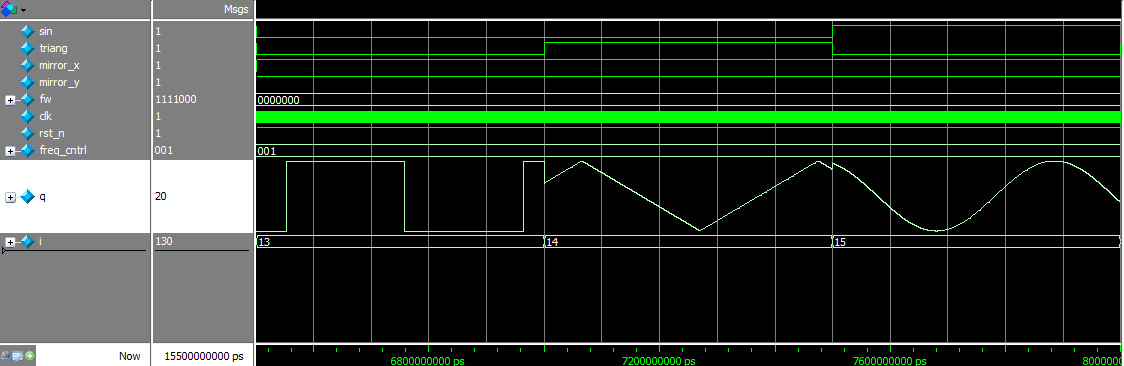
\includegraphics[width=\textwidth]{img/DDFS_outpu_wave.jpg}
    \caption{DDFS testbench output wave}
    \label{fig:DDFS_output_wave}
\end{figure}
\vspace{0.5cm}

\noindent
In \autoref{fig:DDFS_output_wave} are shown the three main waveform with both mirroring effect enabled. \\
The second thing that can be analyzed from the testbench is the variation of the output frequency corresponding to a swing of \texttt{f\_w}.

\vspace{0.5cm}
\begin{figure}[h!]
    \centering
    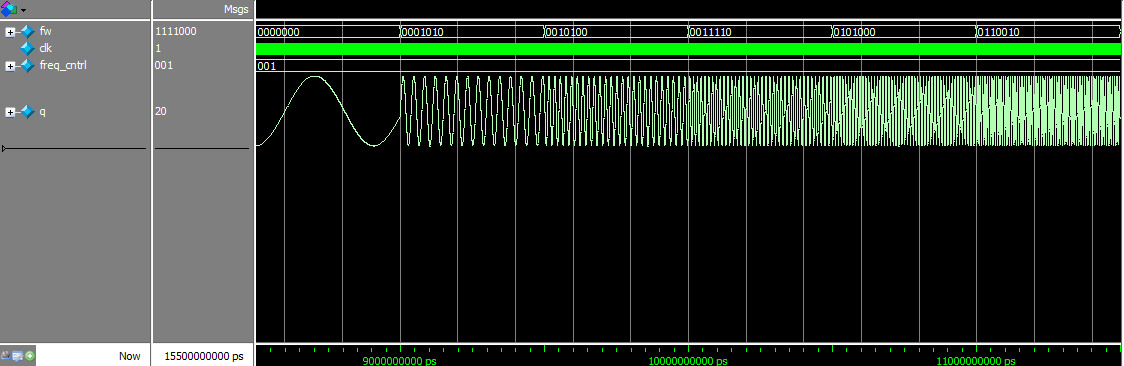
\includegraphics[width=\textwidth]{img/fw_variation_DDFS.jpg}
    \caption{DDFS sine-wave frequency swing}
    \label{fig:fw_variation_DDFS}
\end{figure}
\vspace{0.5cm}
\begin{figure}[h!]
    \centering
    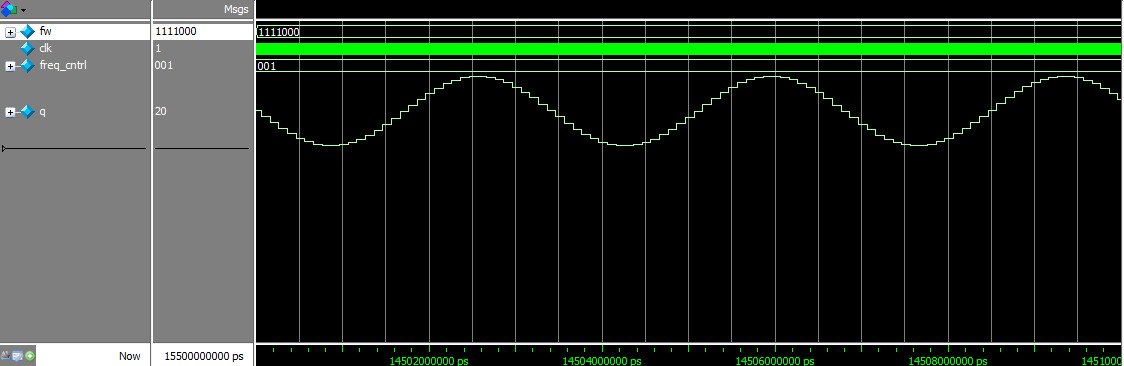
\includegraphics[width=\textwidth]{img/smallest_fw_wave_DDFS.jpg}
    \caption{DDFS sine-wave with biggest value of \texttt{f\_w}}
    \label{fig:smallest_fw_wave_DDFS}
\end{figure}
\vspace{0.5cm}

\noindent
For the frequency divider, only the output frequencies \(\frac{f_{clk}}{2}\), \(\frac{f_{clk}}{10}\), \(\frac{f_{clk}}{100}\), and \(\frac{f_{clk}}{1000}\) were tested, since the other divisions are too large to be simulated.

\vspace{0.5cm}
\begin{figure}[h!]
    \centering
    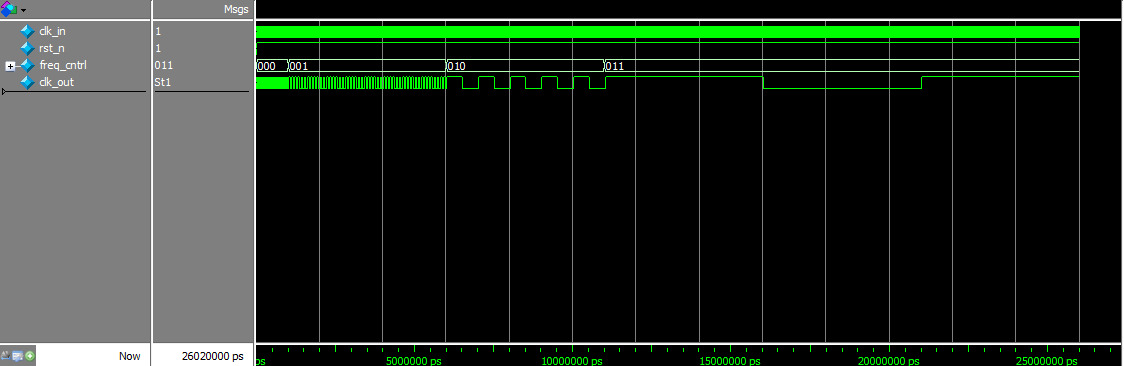
\includegraphics[width=\textwidth]{img/freq_div_DDFS.jpg}
    \caption{DDFS divided frequency from frequency divider}
    \label{fig:freq_div_DDFS}
\end{figure}
\vspace{0.5cm}

\newpage

\subsubsection{Keypad frequency select module}
The test procedure for this module is divided into different parts:  
the test of the keypad module, the test of the frequency converter module, and the test of the modules connected together. \\
To simulate the behavior of the 4×4 matrix keypad (used for the keypad module and for the keypad frequency selection module), a dedicated module has been implemented. \\
This module is controlled via an input bus and simulates the electrical connection between the corresponding columns and rows.

\vspace{1cm}
\begin{lstlisting}[language=Verilog, caption=4x4 keypad simulator module  ]
    module keypad_4x4
    (
        // ---- KEYPAD PINS ---- //
        input [3:0] column,
        output reg [3:0] row,
        
        // ---- BUTTON PINS ---- //
        input [3:0] button,
        input button_pressed
    );
    
        integer i;
        always @(*) begin		
            //assign button value
            if(button_pressed == 1)
                for(i=0; i<4; i=i+1) begin
                    if(i == button/4)
                        row[i] = column[button%4];
                    else
                        row[i] = 1;
                end
            else
                row = 4'b1111;
        end
    
    endmodule
\end{lstlisting}
\vspace{1cm}

\paragraph{Testbench} \quad \\
To test the keypad module, the press of a different keypad button was simulated every \(100ns\), and the values of the \texttt{out\_keys} and \texttt{data\_valid} outputs were read.

\vspace{1cm}
\begin{lstlisting}[language=Verilog, caption=Keypad module testbench  ]
    //none button pressed
    button_pressed = 0;
    
    for(i=0; i<=4'b1111; i=i+1) begin
        //press a button
        #100
        button_pressed = 1;
        button = i;		
    end
    
    //none button pressed
    #100 button_pressed = 0;
\end{lstlisting}
\vspace{1cm}

\noindent
To test the DDFS frequency converter module, the value of the module input frequency was increased from \(0\) to \texttt{MAX\_FREQ}, which was set to \(1MHz\), with a \texttt{CLK\_FREQ} of \(70MHz\). \\
Due to the large range of frequency values, the increment step was set to \(100\).

\vspace{1cm}
\begin{lstlisting}[language=Verilog, caption=DDFS converter module testbench  ]
    for(i=0; i<=MAX_FREQ; i=i+100) begin
        #10 freq = i;
    end
\end{lstlisting}
\vspace{1cm}

\noindent
To test the accuracy of the module with different clock scaling factors, the output waveform frequency was also calculated using the \texttt{f\_w} and \texttt{freq\_cntrl} values processed by the module. \\
Then, the \texttt{delta\_freq} was calculated as the difference between the ideal frequency (the input of the DDFS converter module) and the real frequency (calculated from the output of the DDFS converter module).

\vspace{1cm}
\begin{lstlisting}[language=Verilog, caption=Delta frequency calculation  ]
    reg [63:0] divided_clock;
    always @(*) begin
        case(freq_control)
            
            //select the correct divided_clock output
            3'd0: divided_clock = CLK_FREQ/2;
            3'd1: divided_clock = CLK_FREQ/10;
            3'd2: divided_clock = CLK_FREQ/100;
            3'd3: divided_clock = CLK_FREQ/1000;
            3'd4: divided_clock = CLK_FREQ/10000;
            3'd5: divided_clock = CLK_FREQ/100000;
            3'd6: divided_clock = CLK_FREQ/1000000;
            
            default: begin
                //error stop simulation
                $error("ERROR: frequency divider value out of range");
                $stop;
            end
                
        endcase
    end
    
    assign @(*) begin
    
        if(mirror_x == 0 && mirror_y == 0) begin
            freq_calculated = ((fw+1)*divided_clock)/1024;
        end
        else if(mirror_x == 0 || mirror_y == 0) begin
            freq_calculated = 2*((fw+1)*divided_clock)/1024;
        end
        else begin
            freq_calculated = 4*((fw+1)*divided_clock)/1024;
        end
    
    end
    
    assign delta_freq = freq - freq_calculated;
\end{lstlisting}
\vspace{1cm}

\newpage
\paragraph{Wave analysis} \quad \\
From the keypad module testbench, it is possible to observe the column enabling cycle and the row reading cycle.

\vspace{0.5cm}
\begin{figure}[h!]
    \centering
    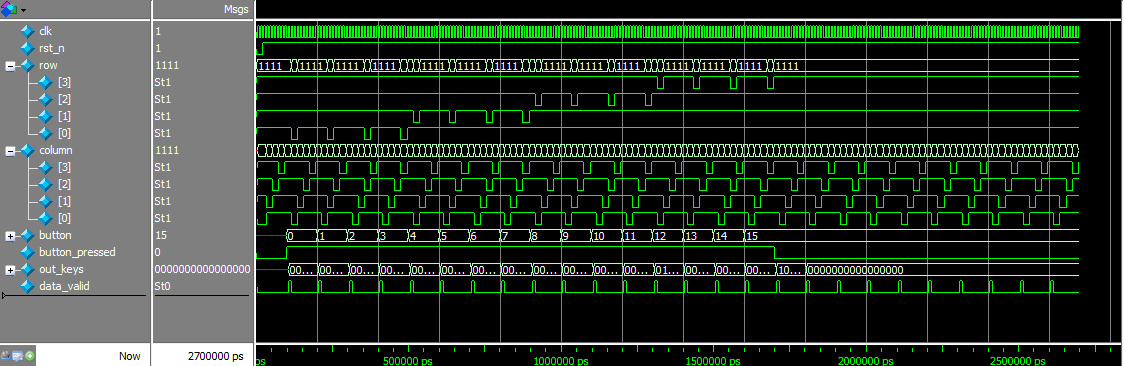
\includegraphics[width=\textwidth]{img/keypad_module_waveform.jpg}
    \caption{Keypad module waveform of scan cycles}
    \label{fig:keypad_module_waveform}
\end{figure}
\vspace{0.5cm}

\noindent
Enabling a column and reading the corresponding rows takes two clock cycles. \\
The output data (rows and column of the button pressed) is sampled and stored into a buffer and at the end of the scanning cycle the value of the buffer is stored into the output vector.

\vspace{0.5cm}
\begin{figure}[h!]
    \centering
    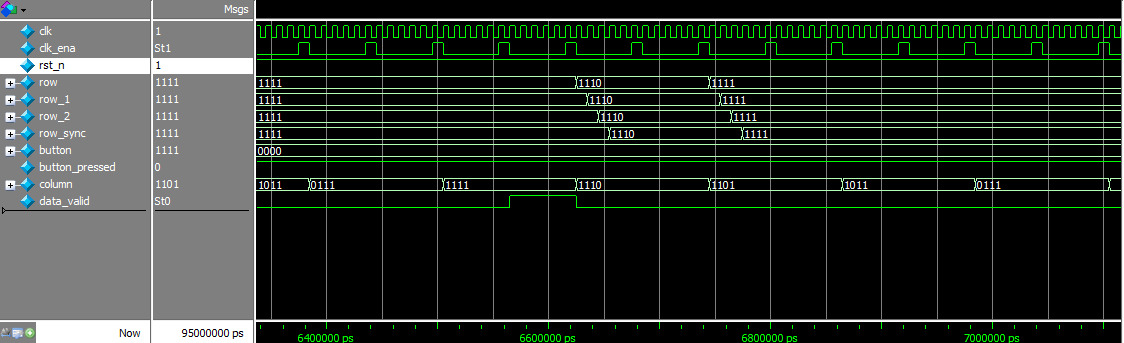
\includegraphics[width=\textwidth]{img/keypad_waveform_detail.jpg}
    \caption{Sampling data of keypad module}
    \label{fig:keypad_waveform_detail}
\end{figure}
\vspace{0.5cm}

\noindent
In \autoref{fig:keypad_waveform_detail} we can see that the row inputs pass through three flip-flops to reduce metastability problems, but this does not cause trouble, because the clock enable rises after \texttt{row\_sync} has stabilized.

\newpage
\noindent
By analyzing the DDFS converter module testbench, we can observe the variation of \texttt{delta\_freq} for a sweep of the input frequency from \(0\,\text{Hz}\) to \(1\,\text{MHz}\), and calculate the maximum absolute (and relative) frequency error for each frequency division (from the frequency divider).

\vspace{0.5cm}
\begin{figure}[h!]
    \centering
    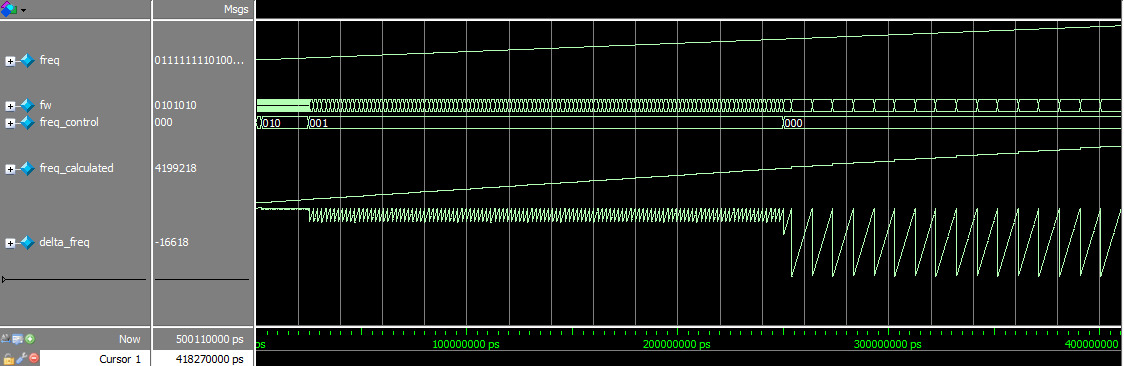
\includegraphics[width=\textwidth]{img/DDFS_freq_wave.jpg}
    \caption{Testbench output of DDFS converter module}
    \label{fig:DDFS_freq_wave}
\end{figure}
\vspace{0.5cm}

\noindent
As we can see in \autoref{fig:DDFS_freq_wave}, the absolute value of \texttt{delta\_freq} is lower than a value that depends on the frequency control calculated by the module. \\
The \texttt{delta\_freq} value is equal to the absolute frequency error.


\begin{itemize}

    \item \(\texttt{freq\_control} = 000\) \\
    \(
        \left|\varepsilon_{a}\right| = \left| f_{in} - f_{measured} \right| < 33000Hz \implies 
        \left|\varepsilon_{r}\right| = \left| \frac{ f_{in} - f_{measured} }{f_{in}} \right| < \left| \frac{ max(\varepsilon_{a}) }{min(f_{in})} \right| \simeq 3.8 \%
    \)
    
    \item \(\texttt{freq\_control} = 001\) \\
    \(
        \left|\varepsilon_{a}\right| = \left| f_{in} - f_{measured} \right| < 6500Hz \implies 
        \left|\varepsilon_{r}\right| = \left| \frac{ f_{in} - f_{measured} }{f_{in}} \right| < \left| \frac{ max(\varepsilon_{a}) }{min(f_{in})} \right| \simeq 7.2 \%
    \)
    
    \item \(\texttt{freq\_control} = 010\) \\
    \(
        \left|\varepsilon_{a}\right| = \left| f_{in} - f_{measured} \right| < 650Hz \implies 
        \left|\varepsilon_{r}\right| = \left| \frac{ f_{in} - f_{measured} }{f_{in}} \right| < \left| \frac{ max(\varepsilon_{a}) }{min(f_{in})} \right| \simeq 7.0 \%
    \)
    
    \item \(\texttt{freq\_control} = 011\) \\
    \(
        \left|\varepsilon_{a}\right| = \left| f_{in} - f_{measured} \right| < 65Hz \implies 
        \left|\varepsilon_{r}\right| = \left| \frac{ f_{in} - f_{measured} }{f_{in}} \right| < \left| \frac{ max(\varepsilon_{a}) }{min(f_{in})} \right| \simeq 7.1 \%
    \)

    \item \(\texttt{freq\_control} = 100\) \\
    \(
        \left|\varepsilon_{a}\right| = \left| f_{in} - f_{measured} \right| < 6Hz \implies 
        \left|\varepsilon_{r}\right| = \left| \frac{ f_{in} - f_{measured} }{f_{in}} \right| < \left| \frac{ max(\varepsilon_{a}) }{min(f_{in})} \right| \simeq 6.7 \%
    \)

    \item \(\texttt{freq\_control} = 101\) \\
    \(
        \left|\varepsilon_{a}\right| = \left| f_{in} - f_{measured} \right| < 1Hz \implies 
        \left|\varepsilon_{r}\right| = \left| \frac{ f_{in} - f_{measured} }{f_{in}} \right| < \left| \frac{ max(\varepsilon_{a}) }{min(f_{in})} \right| \simeq 0 \%
    \)

    \item \(\texttt{freq\_control} = 110\) \\
    \(
        \left|\varepsilon_{a}\right| = \left| f_{in} - f_{measured} \right| = 0Hz \implies 
        \left|\varepsilon_{r}\right| = \left| \frac{ f_{in} - f_{measured} }{f_{in}} \right| = 0\%
    \)
    
\end{itemize}

\newpage

\subsubsection{LCD module}
We want to test the correct states change of the two FSM of the LCD module. 

\paragraph{Testbench} \quad \\
Only for simulation purposes the delays needed to drive the LCD are reduced to a fixed value of 40 ns, this way it is simpler to test the module with Modelsim. To solve this scope a testing Verilog file is created (\texttt{lcd\_driver\_test.v})

\vspace{0.5cm}
\begin{lstlisting}[language=Verilog, caption=LCD module testbench  ]
    initial begin
        reset_n = 1'b0;
        button_next = 1'b1;
        button_prev = 1'b1;
        bcd_freq = 28'hFFFFFFF;
        
        #(CLK_PERIOD*2)	  
        reset_n = 1'b1;
        
        #(CLK_PERIOD*2000)
        button_next = 1'b0;
        
        #(CLK_PERIOD*10)
        button_next = 1'b1;
        
        #(CLK_PERIOD*1000)
        button_next = 1'b0;
        
        #(CLK_PERIOD*10)
        button_next = 1'b1;
        
        #(CLK_PERIOD*1000)
        button_prev = 1'b0;
        
        #(CLK_PERIOD*10)
        button_prev = 1'b1;
            
        #(CLK_PERIOD*1000)
        // Finish simulation
        $stop;
    end
\end{lstlisting}
\vspace{1cm}

\newpage

\paragraph{Wave analysis} \quad \\
The simulation starts with a reset and after that the \texttt{POWER\_ON} state is enabled, followed by the first writing cycle to the LCD. As we can see, at first, in the \texttt{lcd\_data} register is stored the first instruction present in the LUT to send to the LCD (hex38, initializing the function set), then when the first writing cycle is completed the next instruction is read from the LUT and loaded in the \texttt{lcd\_data} register. 

\vspace{0.5cm}
\begin{figure}[h!]
    \centering
    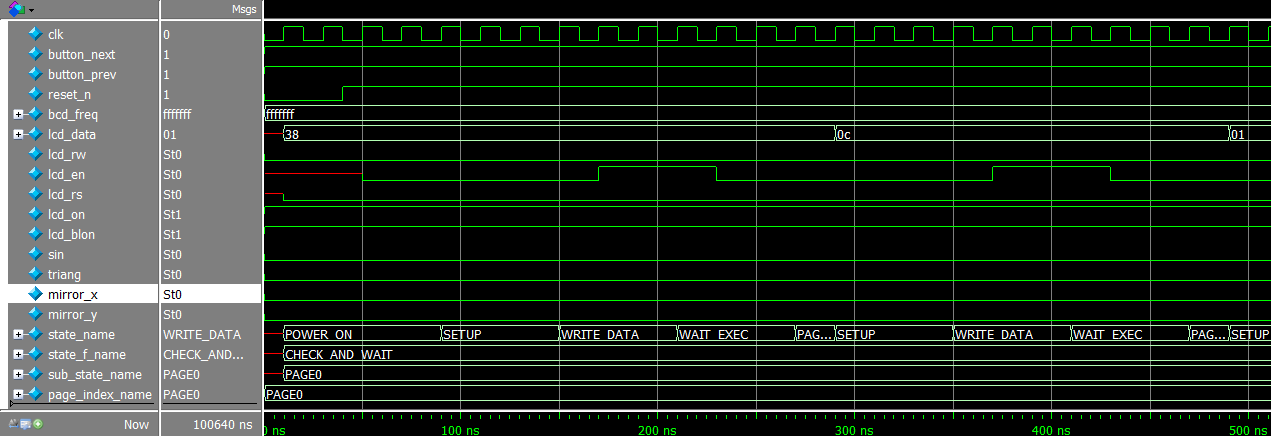
\includegraphics[width=\textwidth]{img/LCD_module_wave1.png}
    \caption{LCD power on}
    \label{fig:LCD_module_wave1}
\end{figure}
\vspace{0.5cm}

\noindent
After sending the first instruction to initialize the LCD we can start to send ASCII characters by setting the register select flag to 1. In \autoref{fig:LCD_module_wave2} we see the ASCII coded characters that are written to the DDRAM of the LCD, each in sequence with a writing cycle. 

\vspace{0.5cm}
\begin{figure}[h!]
    \centering
    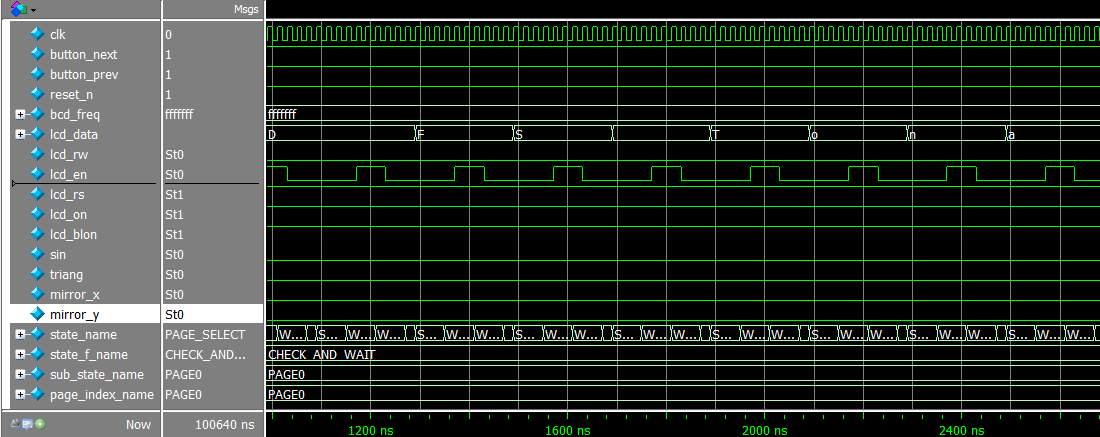
\includegraphics[width=\textwidth]{img/LCD_module_wave2.png}
    \caption{Displaying characters}
    \label{fig:LCD_module_wave2}
\end{figure}
\vspace{0.5cm}

\newpage

\noindent
When a page is completely displayed the first FSM enters the \texttt{WAIT\_BUTTON\_SHORT} state, waiting for the button to be pressed and released. At this point the second FSM is activated, displaying the frequency digits received as BCD input vector in the second row of the display (\autoref{fig:LCD_module_wave3}).  

\vspace{0.5cm}
\begin{figure}[h!]
    \centering
    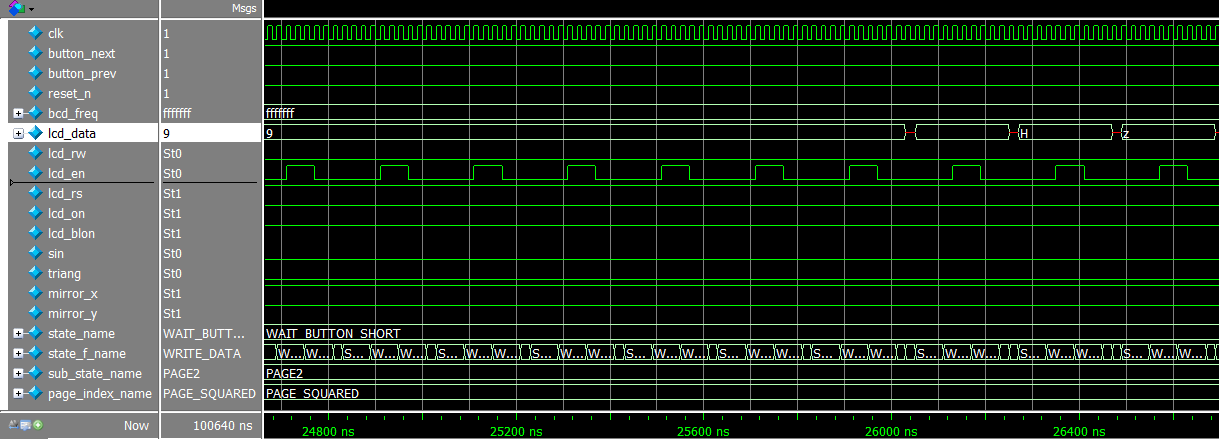
\includegraphics[width=\textwidth]{img/LCD_module_wave3.png}
    \caption{Displaying frequency digits}
    \label{fig:LCD_module_wave3}
\end{figure}
\vspace{0.5cm}

\noindent
In the example in \autoref{fig:LCD_module_wave4} the button is pressed to change the wave function to display, changing from squared wave to triangular wave, the output \texttt{triang} is enabled to signal the new waveform to the DDFS module. Since a new page with new characters needs to be displayed, a new writing cycle of the first FSM starts, the second FSM starts waiting until the first FSM has completed the job (entering the \texttt{WAIT\_BUTTON\_SHORT} state again).  

\vspace{0.5cm}
\begin{figure}[h!]
    \centering
    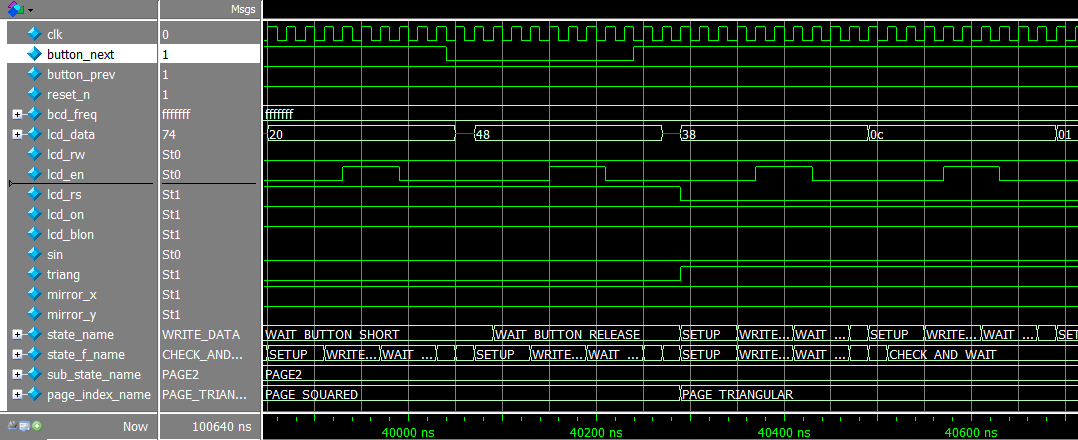
\includegraphics[width=\textwidth]{img/LCD_module_wave4.png}
    \caption{Changing wave function}
    \label{fig:LCD_module_wave4}
\end{figure}
\vspace{0.5cm}

\newpage

\subsection{On-board module testing}
To verify that each module works properly on the board, each module has been tested individually on the board, using the keys, buttons, and LEDs present on the \textbf{Altera DE2 development board}.

\subsubsection{DDFS module}

\vspace{0.5cm}
\begin{figure}[h!]
    \centering
    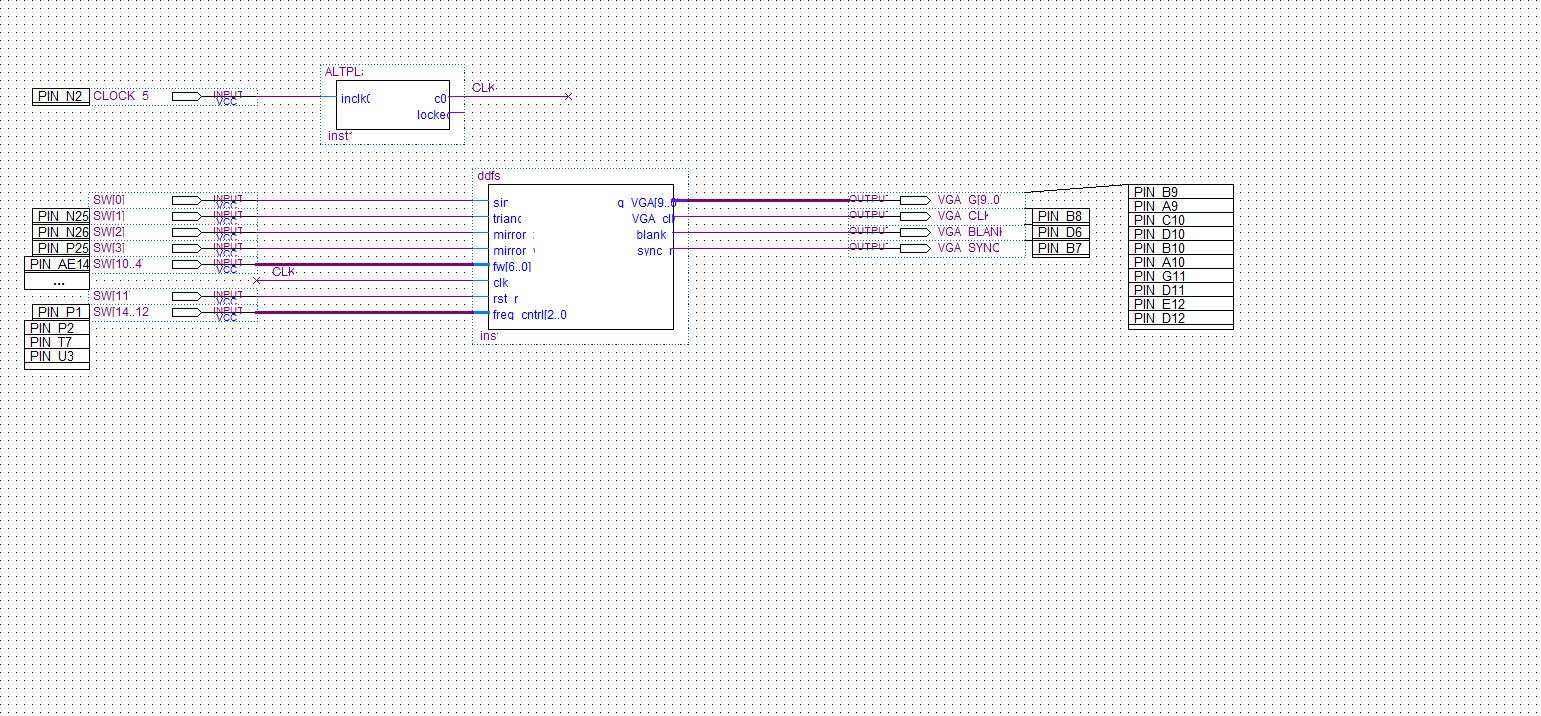
\includegraphics[width=\textwidth]{img/DDFS_onboard_test.jpg}
    \caption{DDFS onboard test schematic}
    \label{fig:DDFS_onboard_test}
\end{figure}
\vspace{0.5cm}

\noindent
As we can see from \autoref{fig:DDFS_onboard_test}, the module inputs have been connected to the keys on the board.\\
The output has been connected to the VGA DAC inputs.\\
The input \(50MHz\) clock source from the board passes through the internal PLL of the FPGA and becomes a \(70MHz\) clock signal. \\
The oscilloscope can be connected to the green channel of the VGA port to monitor the analog output signal of the waveform generator and verify that the output matches the module's input.

\newpage

\subsubsection{Keypad frequency select module}

\vspace{0.5cm}
\begin{figure}[h!]
    \centering
    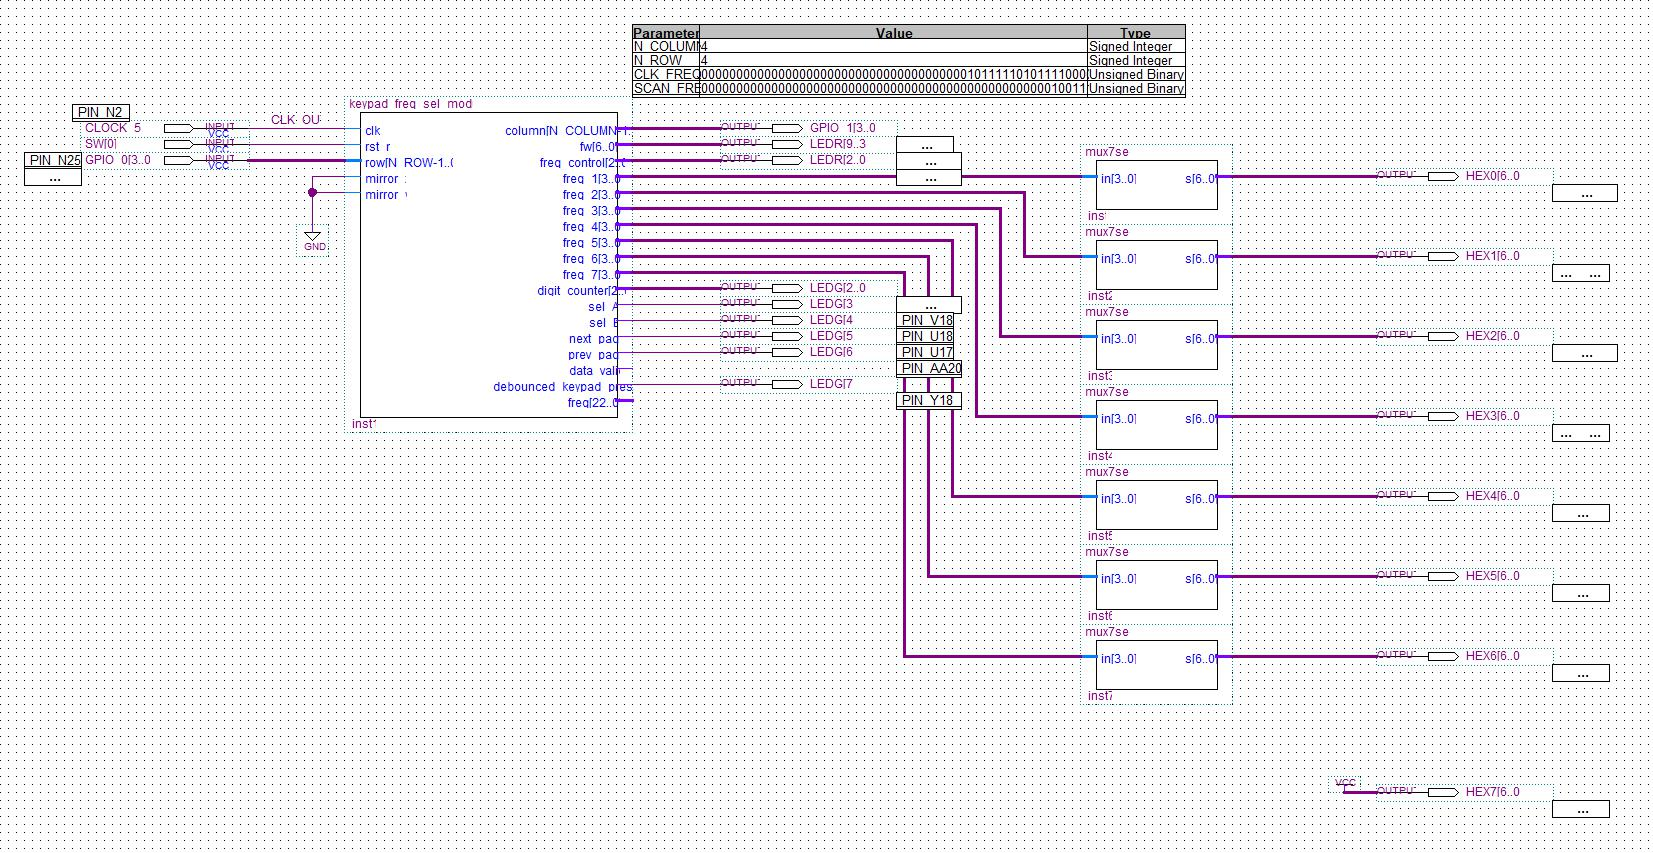
\includegraphics[width=\textwidth]{img/keypad_freq_sel_onboard_test.jpg}
    \caption{keypad frequency select onboard test schematic}
    \label{fig:keypad_freq_sel_onboard_test}
\end{figure}
\vspace{0.5cm}

\noindent
The pins of the keypad have been connected to the GPIO of the board, and the input pins must be configured as input pull-up. \\
The output of the module has been connected, through a BCD-to-7-segment display converter module, to the 7-segment displays on the board, to control the digit shift and the selection of the output signal. \\
The clock source comes from the oscillator on the board but the module work with a clock enable signal, to match the frequency scan value (an external parameter). \\
The other control pins for the DDFS module are connected to the remaining LEDs on the board.

\newpage

\subsubsection{LCD module}

\vspace{0.5cm}
\begin{figure}[h!]
    \centering
    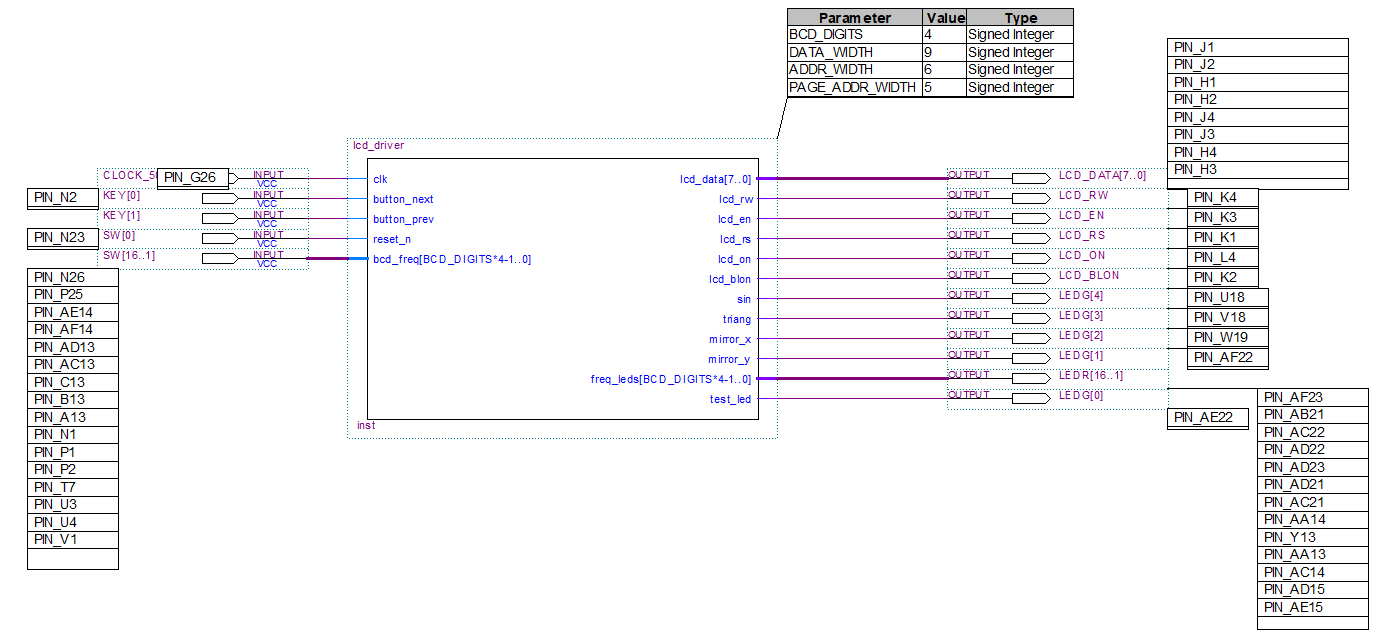
\includegraphics[width=\textwidth]{img/LCD_module_assignment.png}
    \caption{LCD module onboard test schematic}
    \label{fig:LCD_module_assignment}
\end{figure}
\vspace{0.5cm}

\noindent
In the testing phase of the LCD module it has been useful to connect the inputs of the \texttt{bcd\_freq} vector to 16 switches of the board to display at least 4 variable digits (4 switches for each BCD digit), the button for the next and previous page were connected to two physical buttons of the board, and LEDs were used to show the outputs (sin, triang, mirror\_x, mirror\_y) and to test the buttons and switch activation (test\_led, freq\_leds). 

\newpage
\subsubsection{Physical test of the entire design}
In this section some examples and capabilities of the final design are shown.

\vspace{0.5cm}
\begin{figure}[h!]
    \centering
    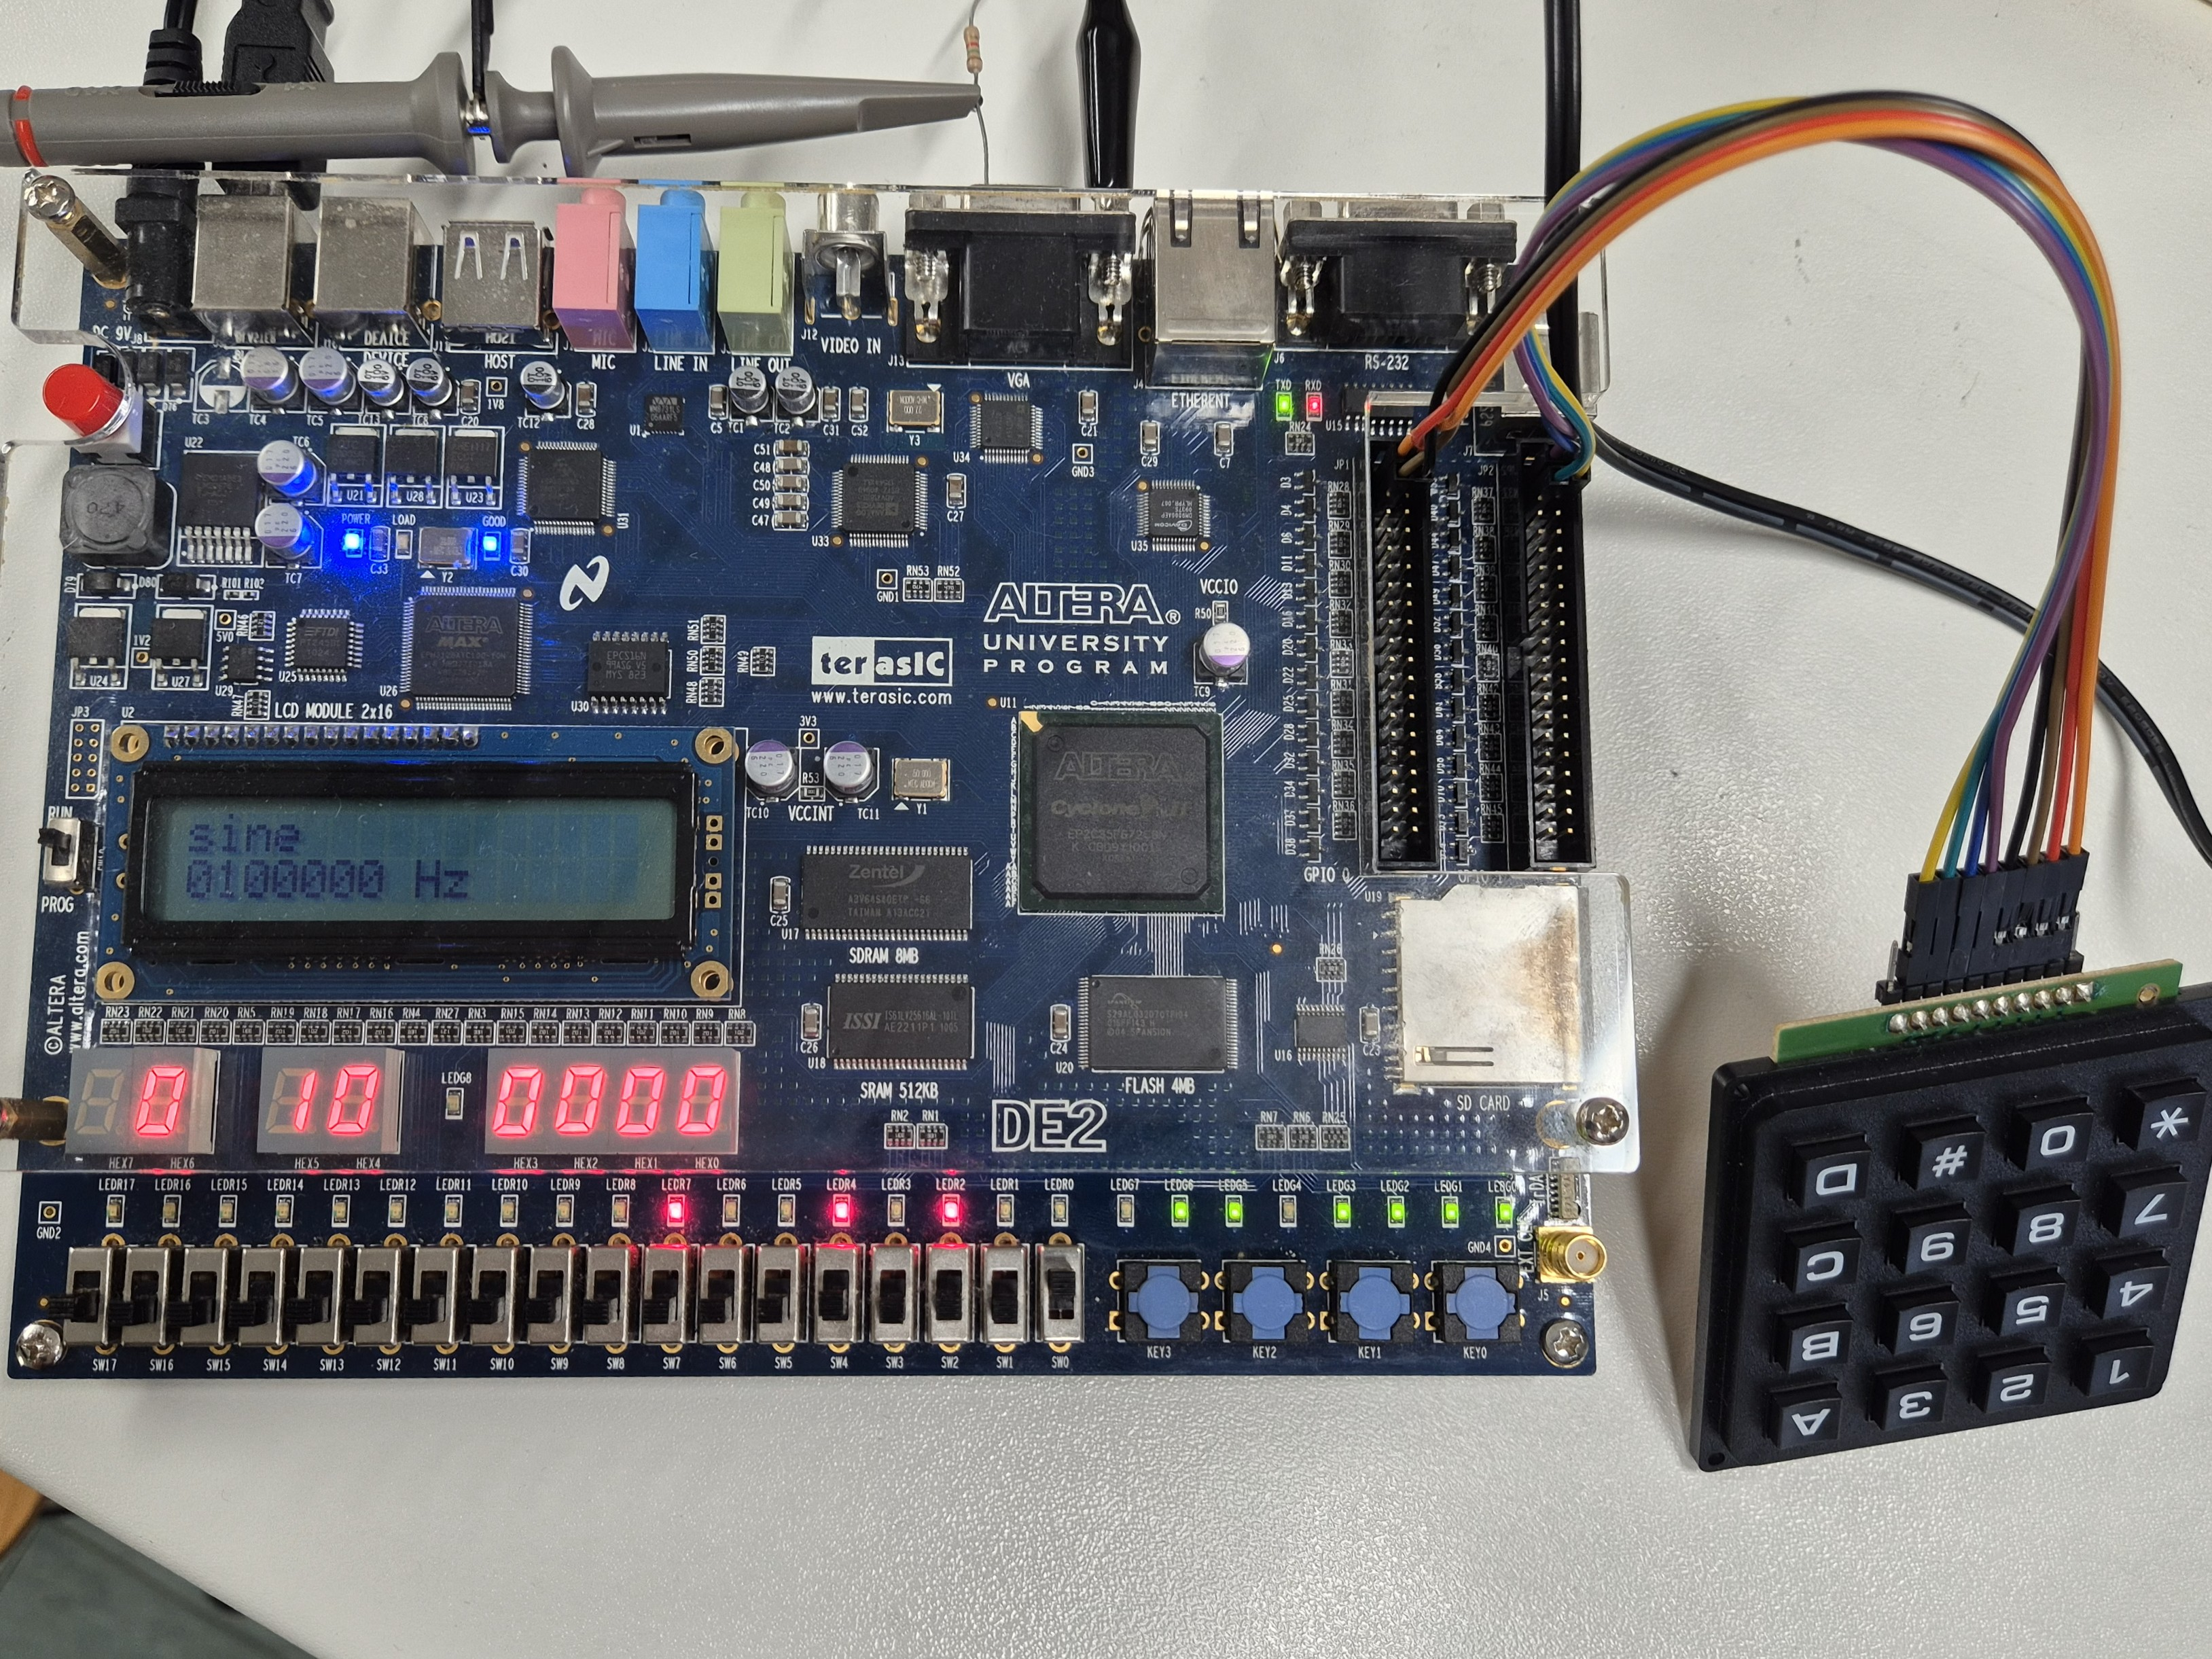
\includegraphics[width=0.8\textwidth]{img/final_test_img7.jpg}
    \caption{Selecting the sine wave with a 100kHz frequency}
    \label{fig:final_test_img7}
\end{figure}

\begin{figure}[h!]
    \centering
    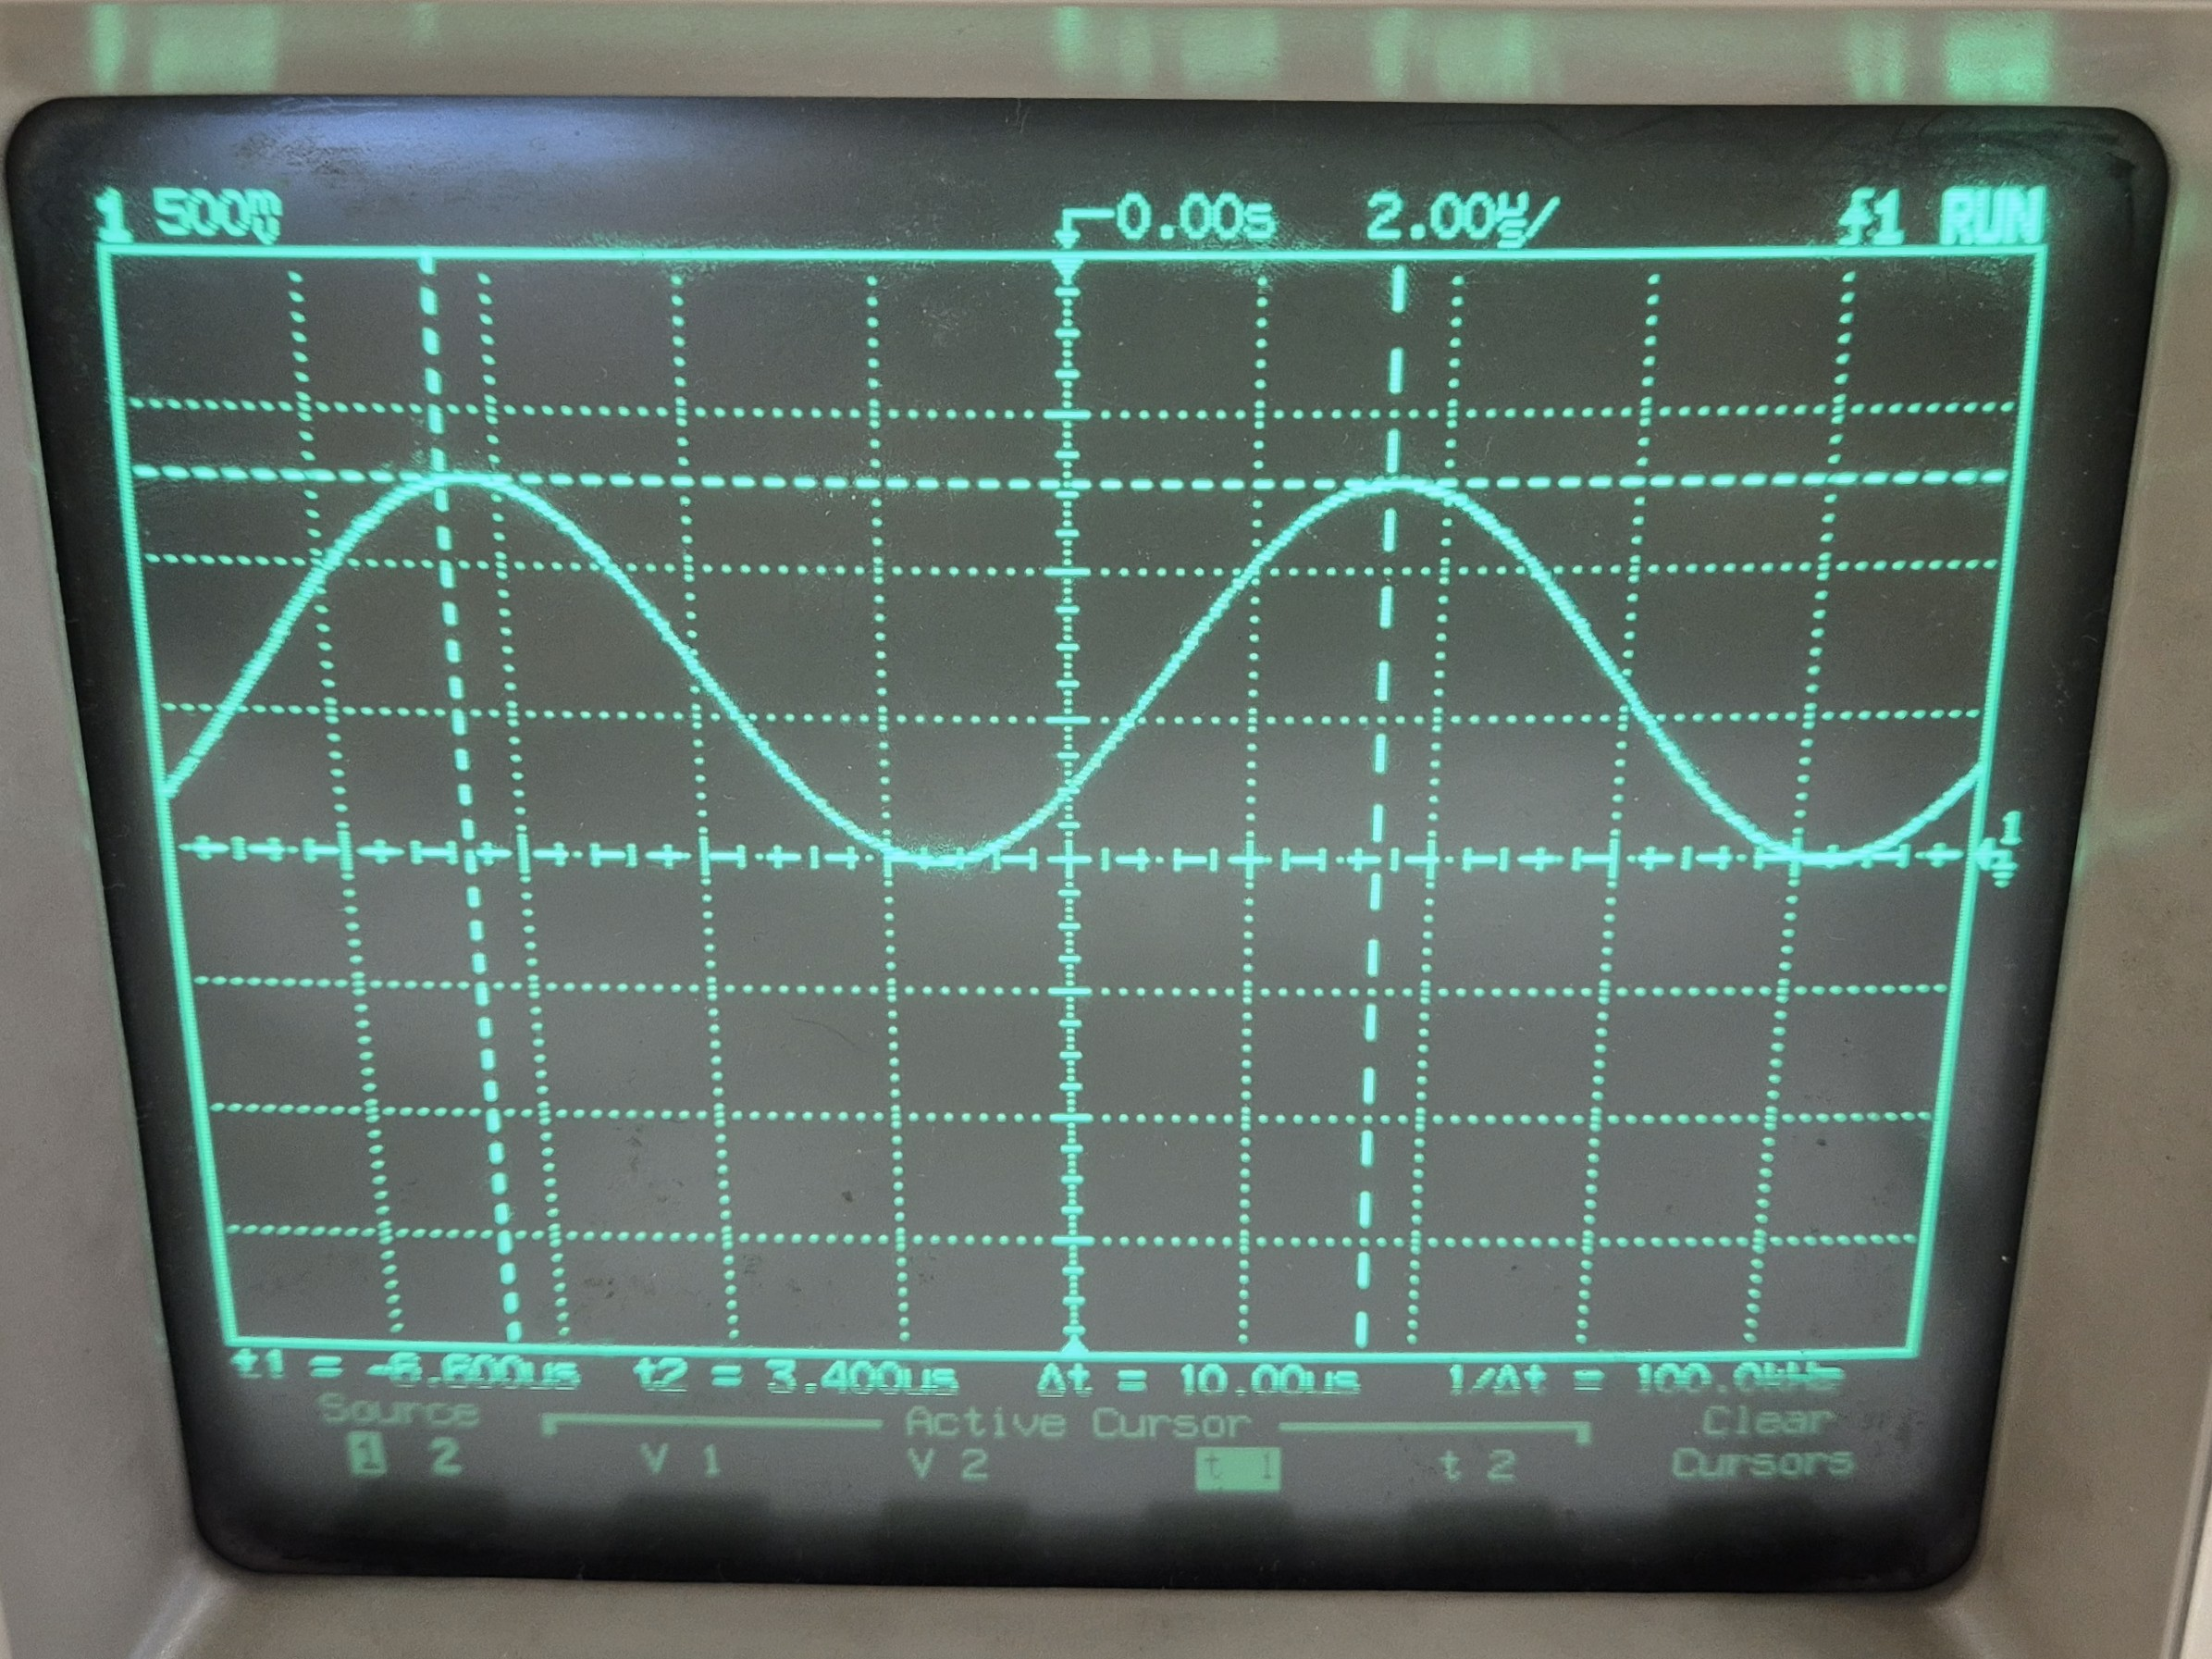
\includegraphics[width=0.8\textwidth]{img/final_test_img8.jpg}
    \caption{Sine wave, oscilloscope view}
    \label{fig:final_test_img8}
\end{figure}

\newpage

\begin{figure}[h!]
    \centering
    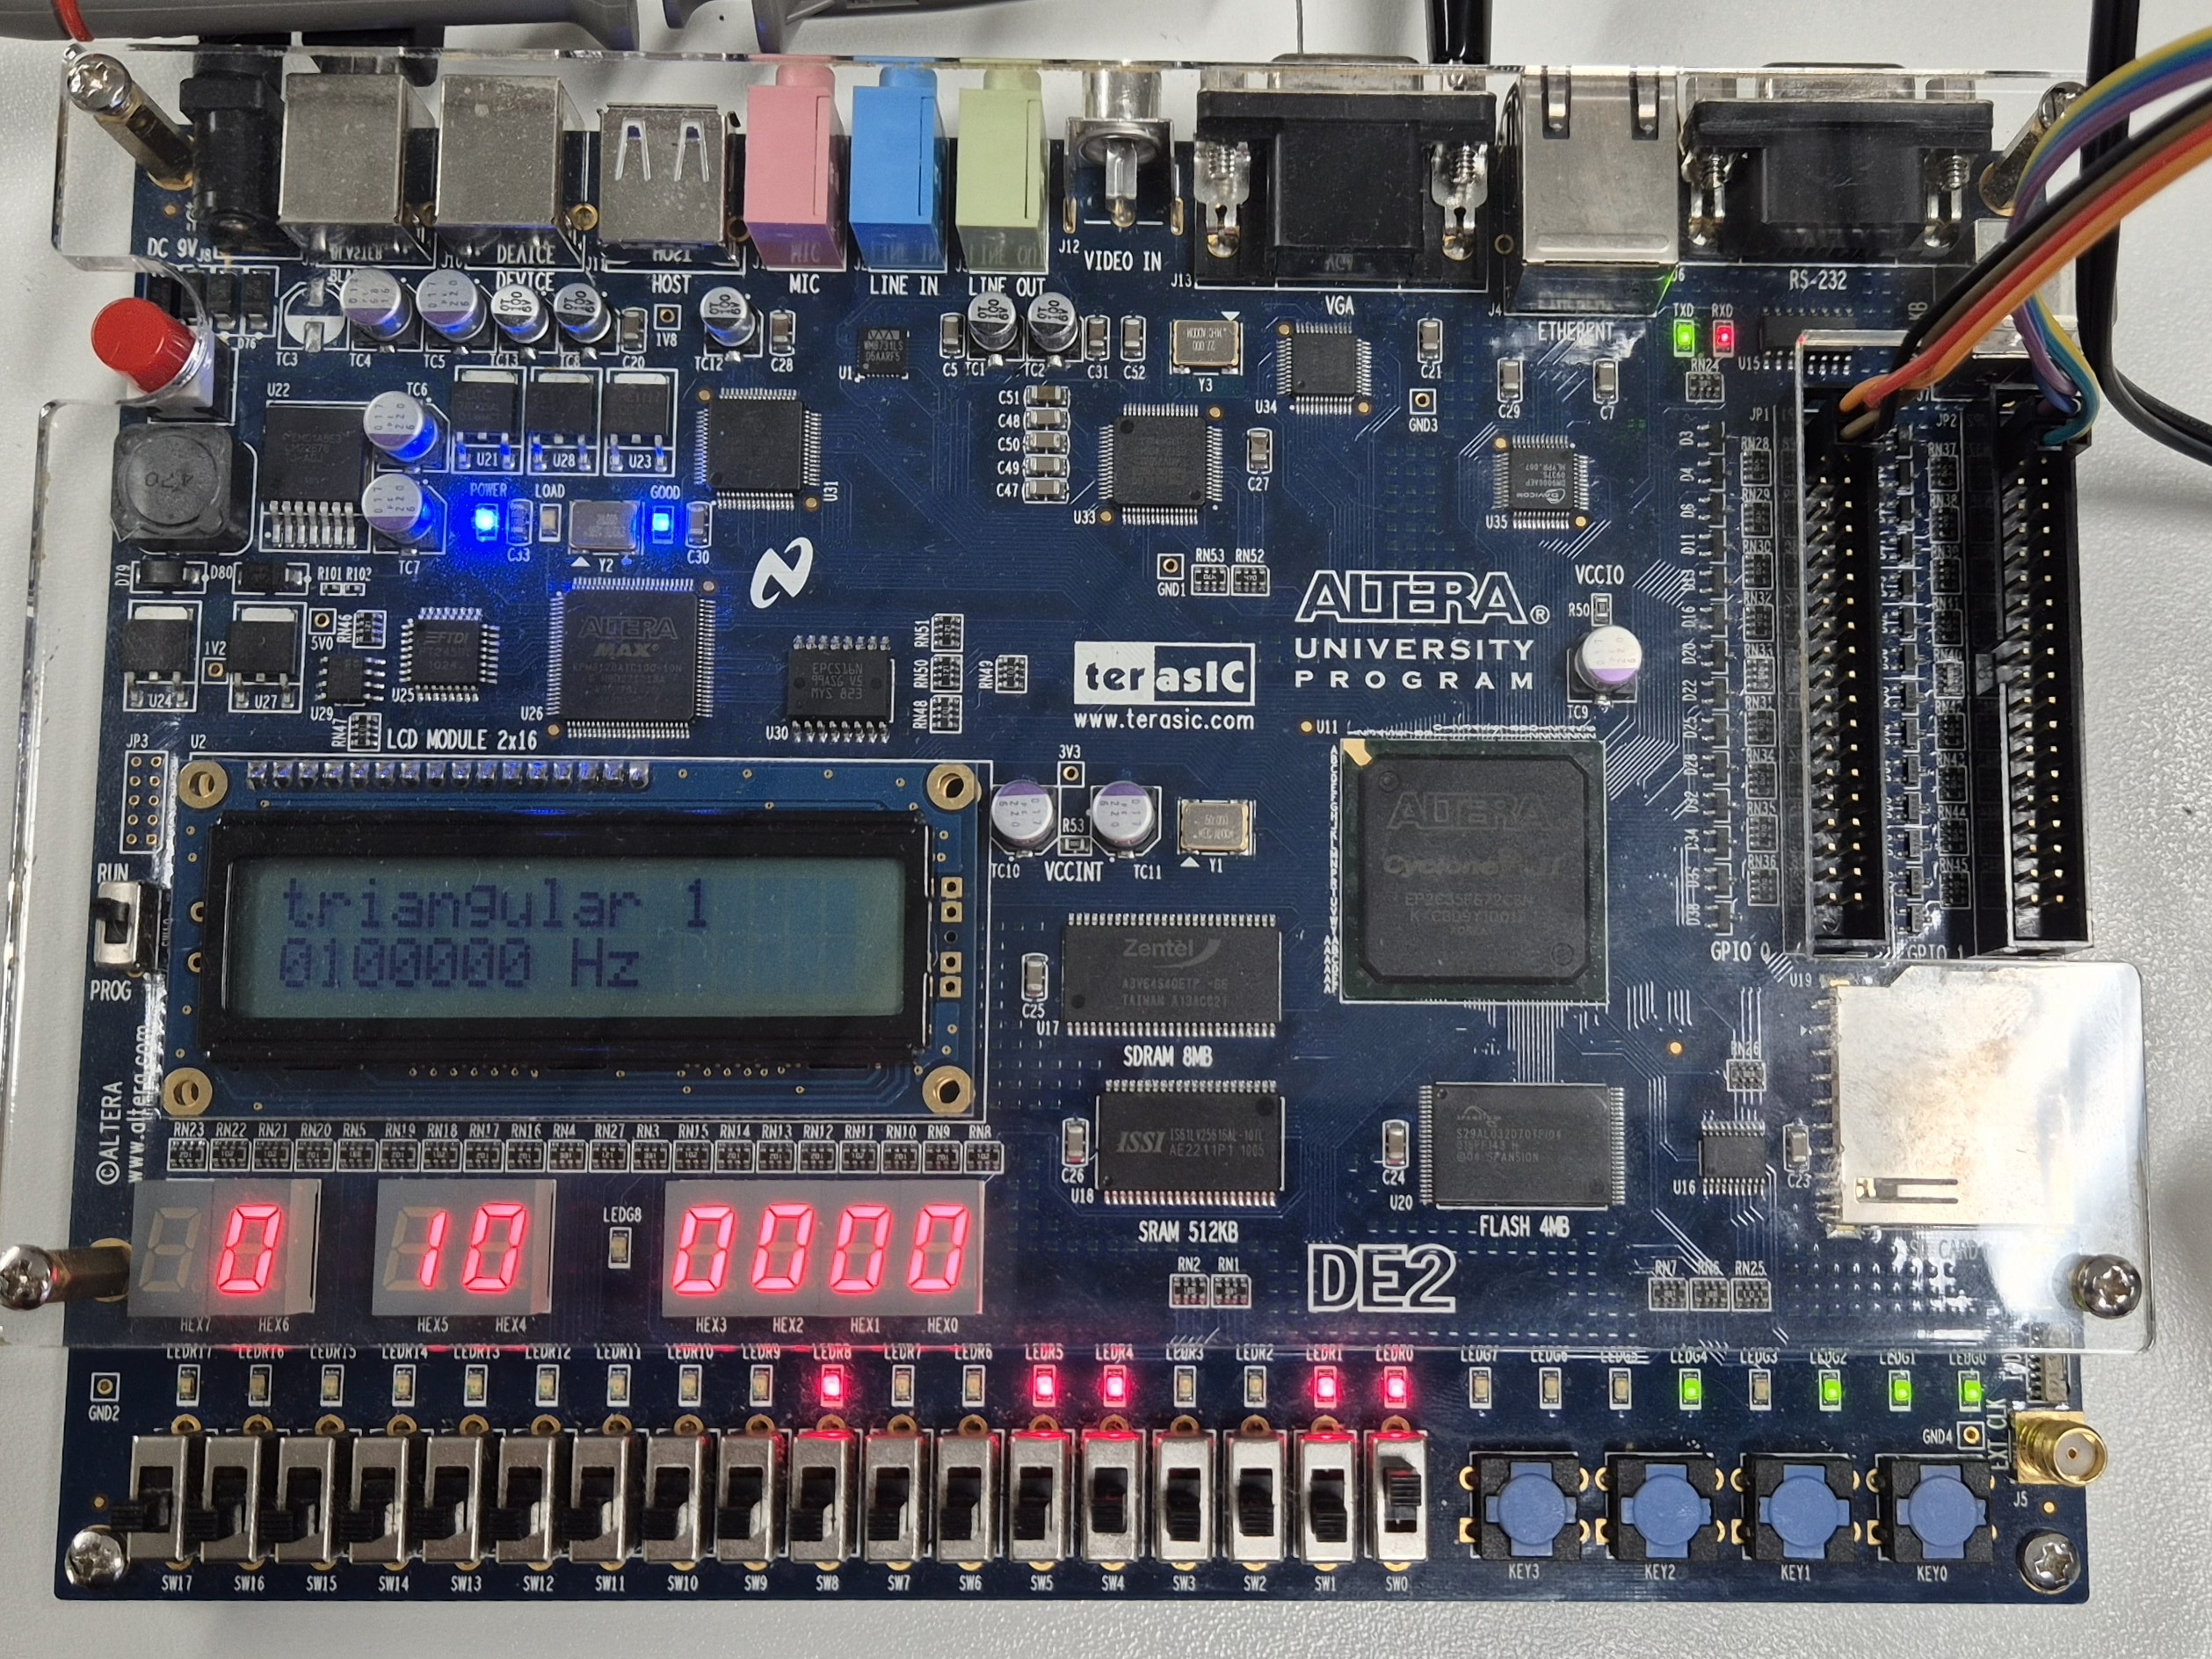
\includegraphics[width=0.8\textwidth]{img/final_test_img3.jpg}
    \caption{Selecting the sawtooth wave with a 100kHz frequency}
    \label{fig:final_test_img3}
\end{figure}

\begin{figure}[h!]
    \centering
    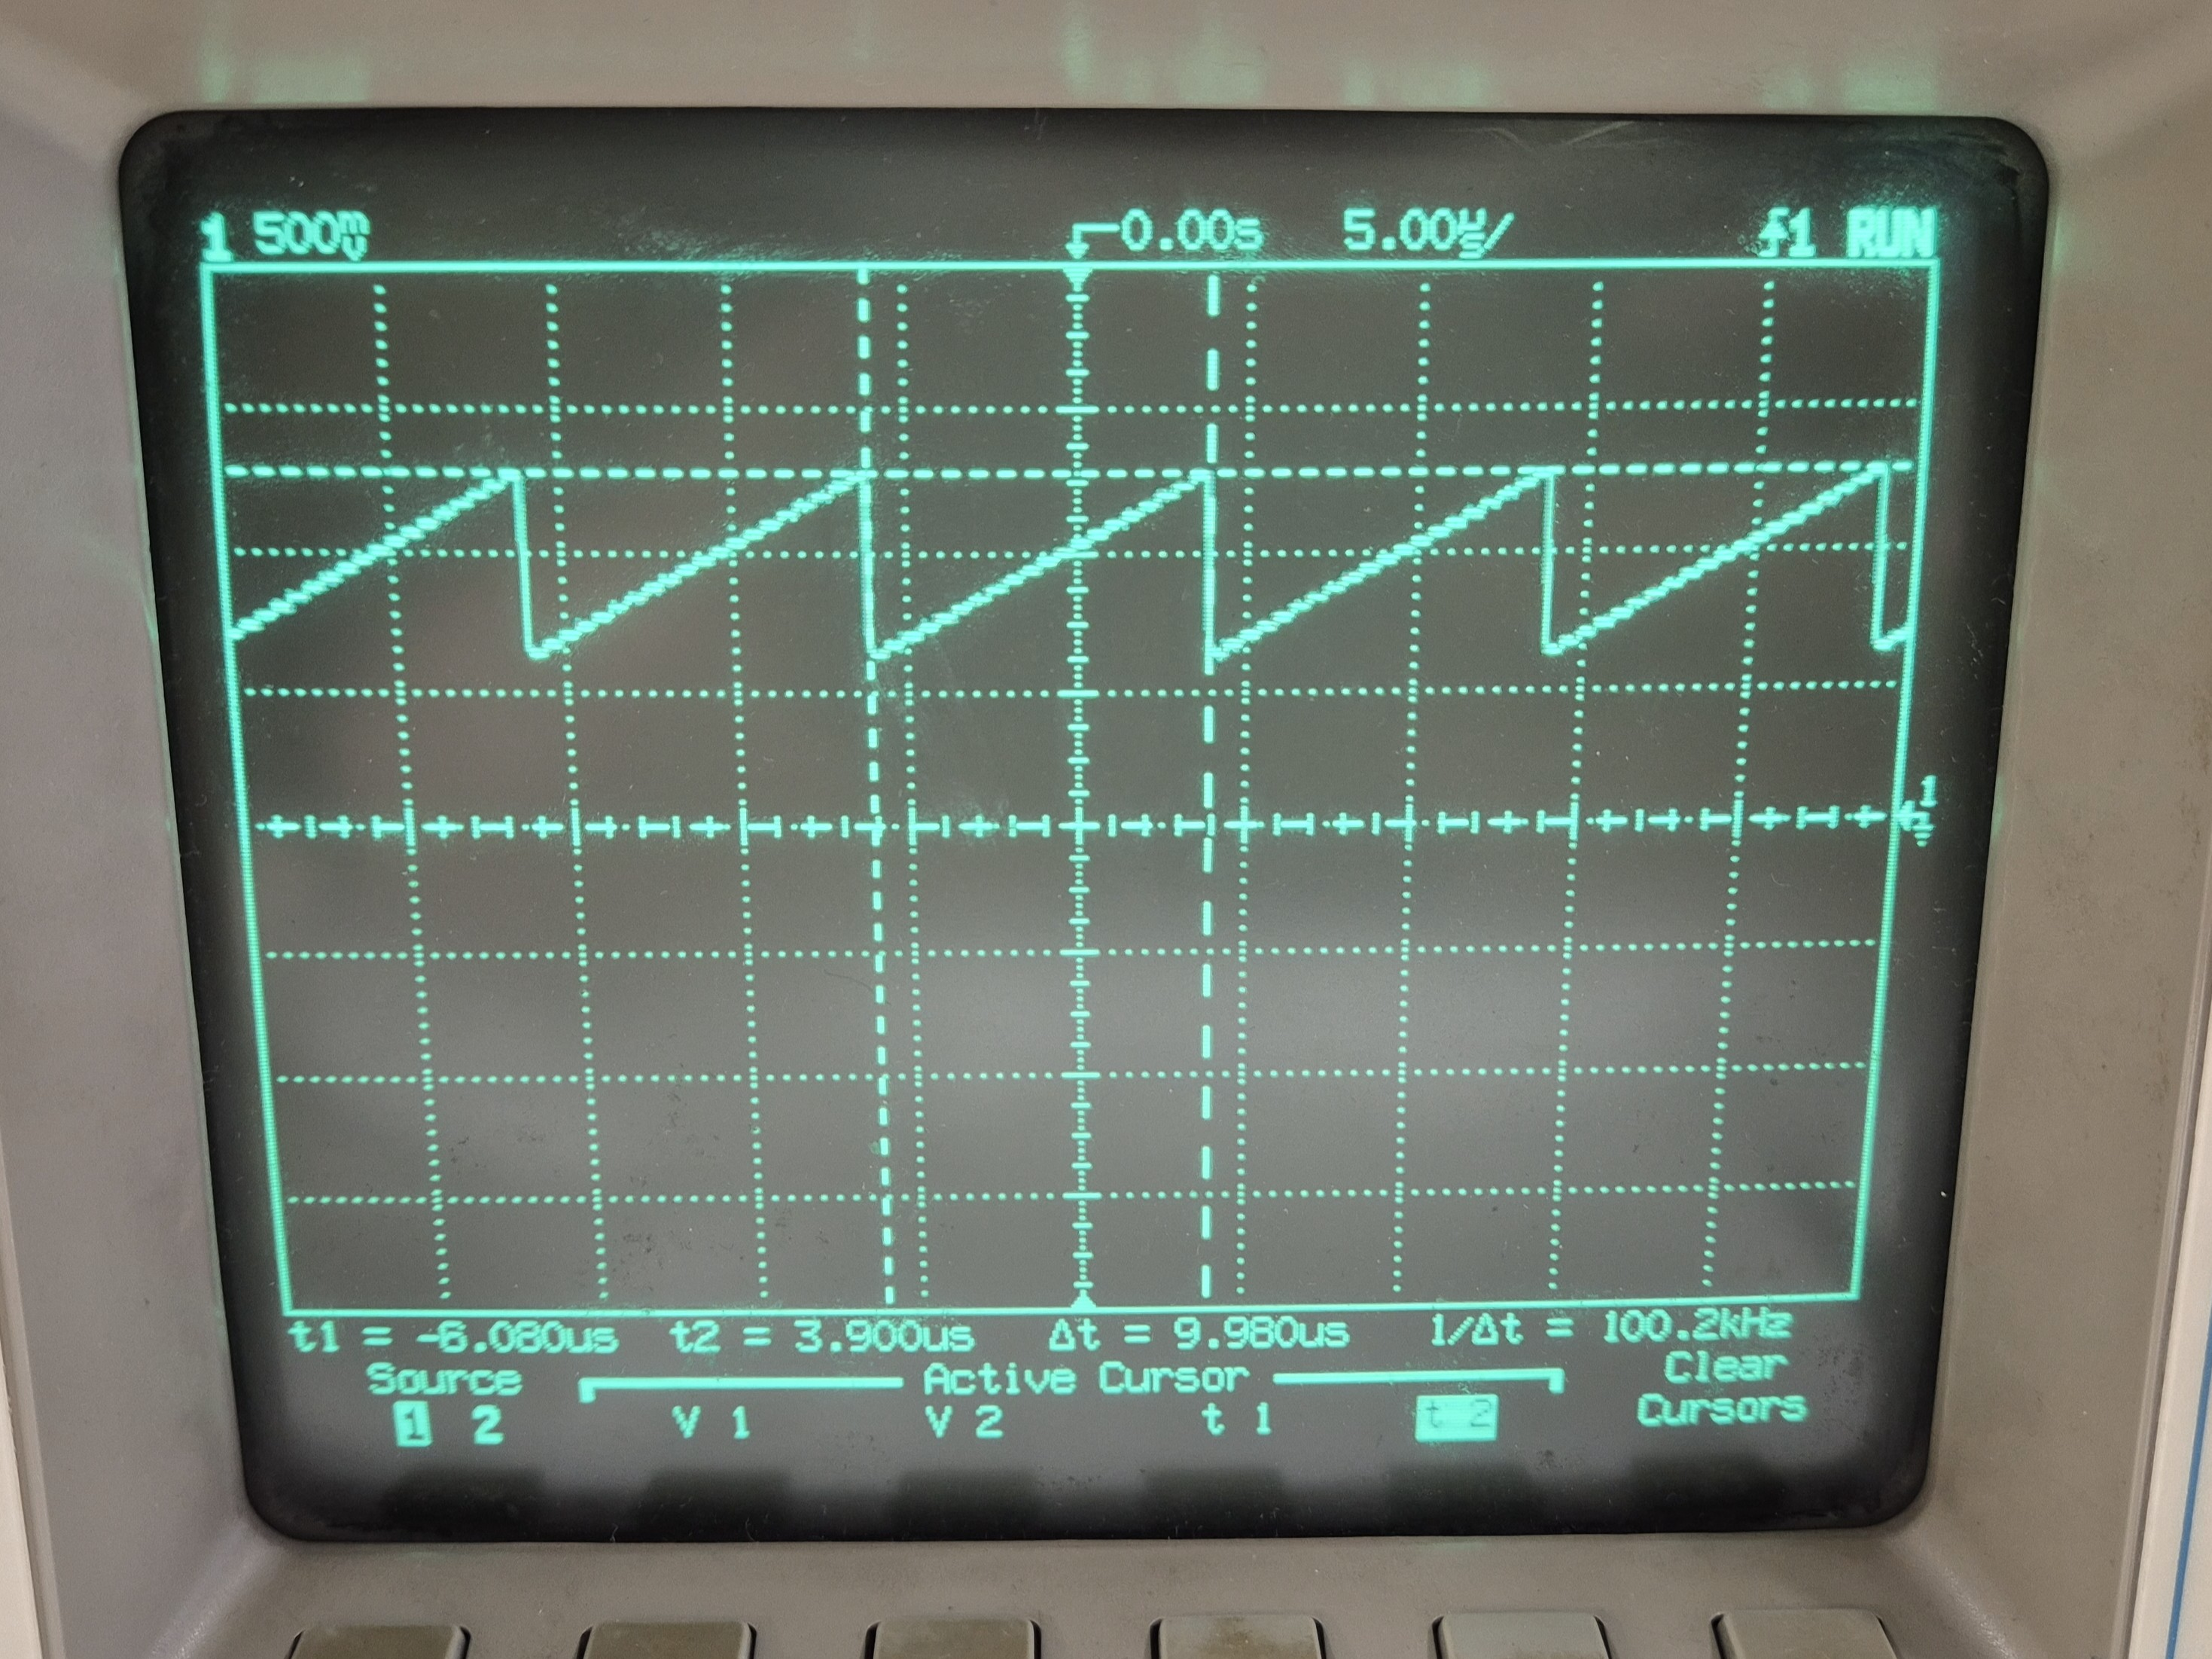
\includegraphics[width=0.8\textwidth]{img/final_test_img4.jpg}
    \caption{Sawtooth wave, oscilloscope view}
    \label{fig:final_test_img4}
\end{figure}

\newpage

\begin{figure}[h!]
    \centering
    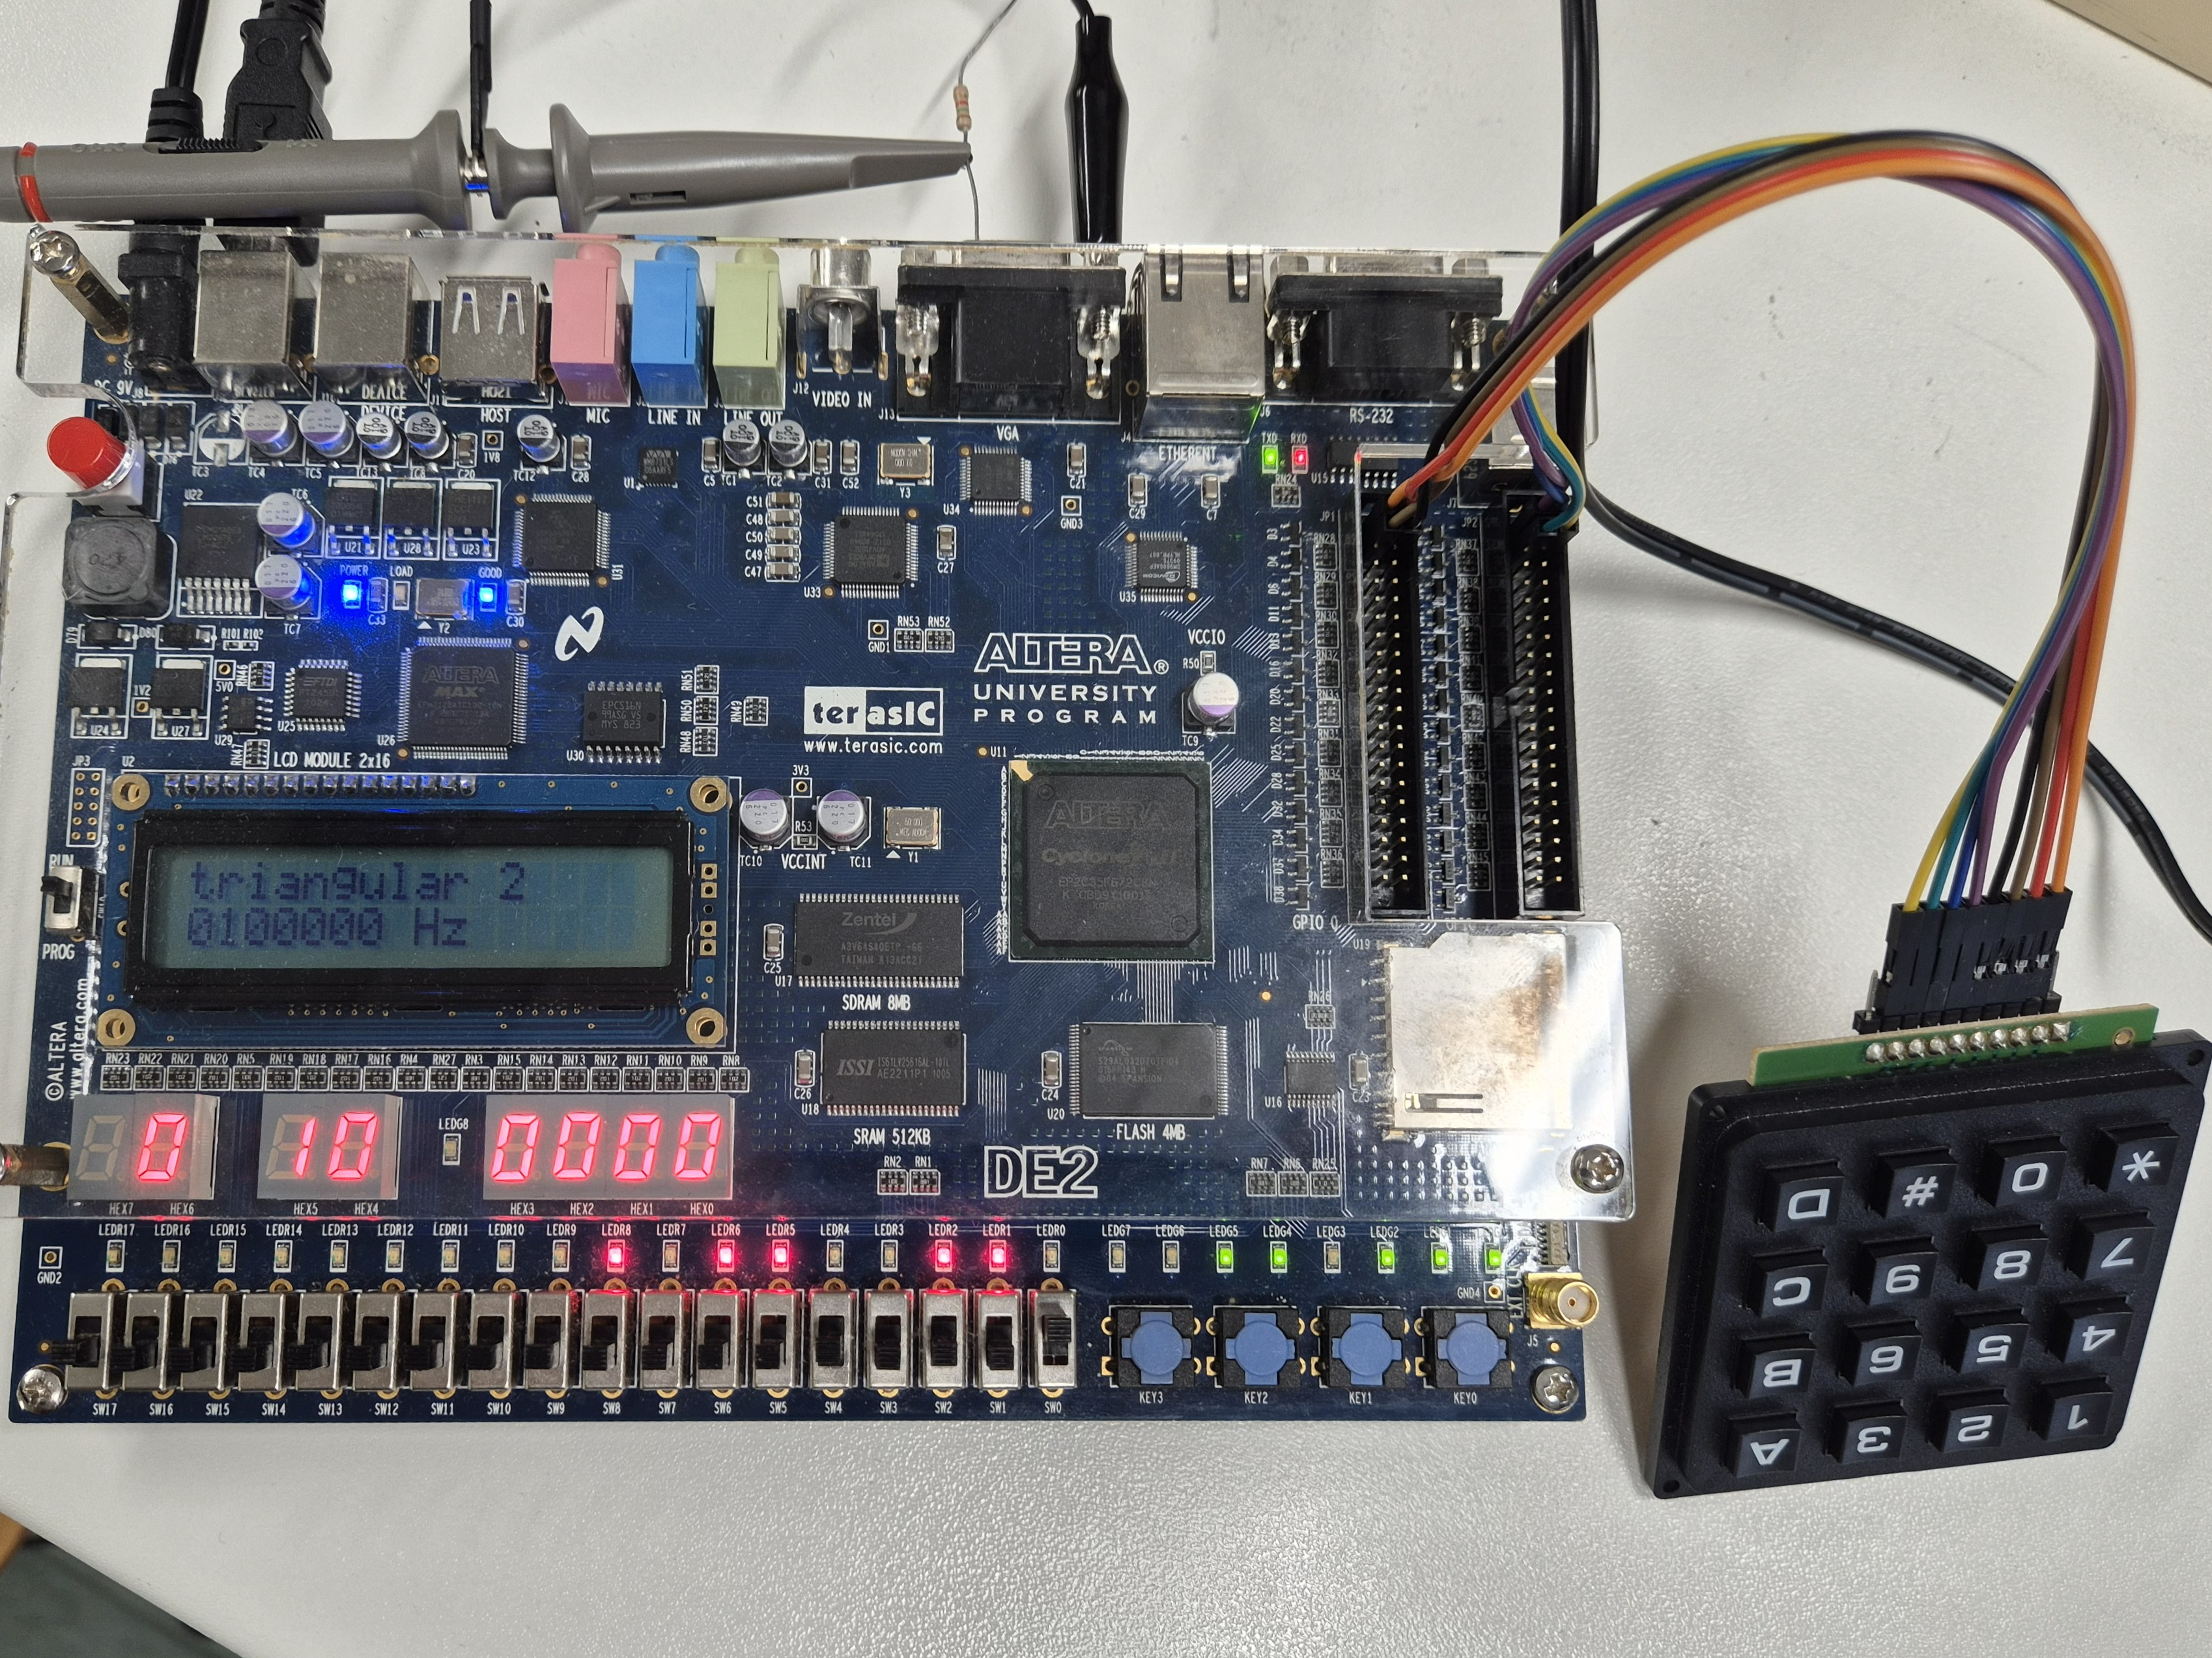
\includegraphics[width=0.8\textwidth]{img/final_test_img5.jpg}
    \caption{Quarter triangular x mirrored with a 100kHz frequency}
    \label{fig:final_test_img5}
\end{figure}

\begin{figure}[h!]
    \centering
    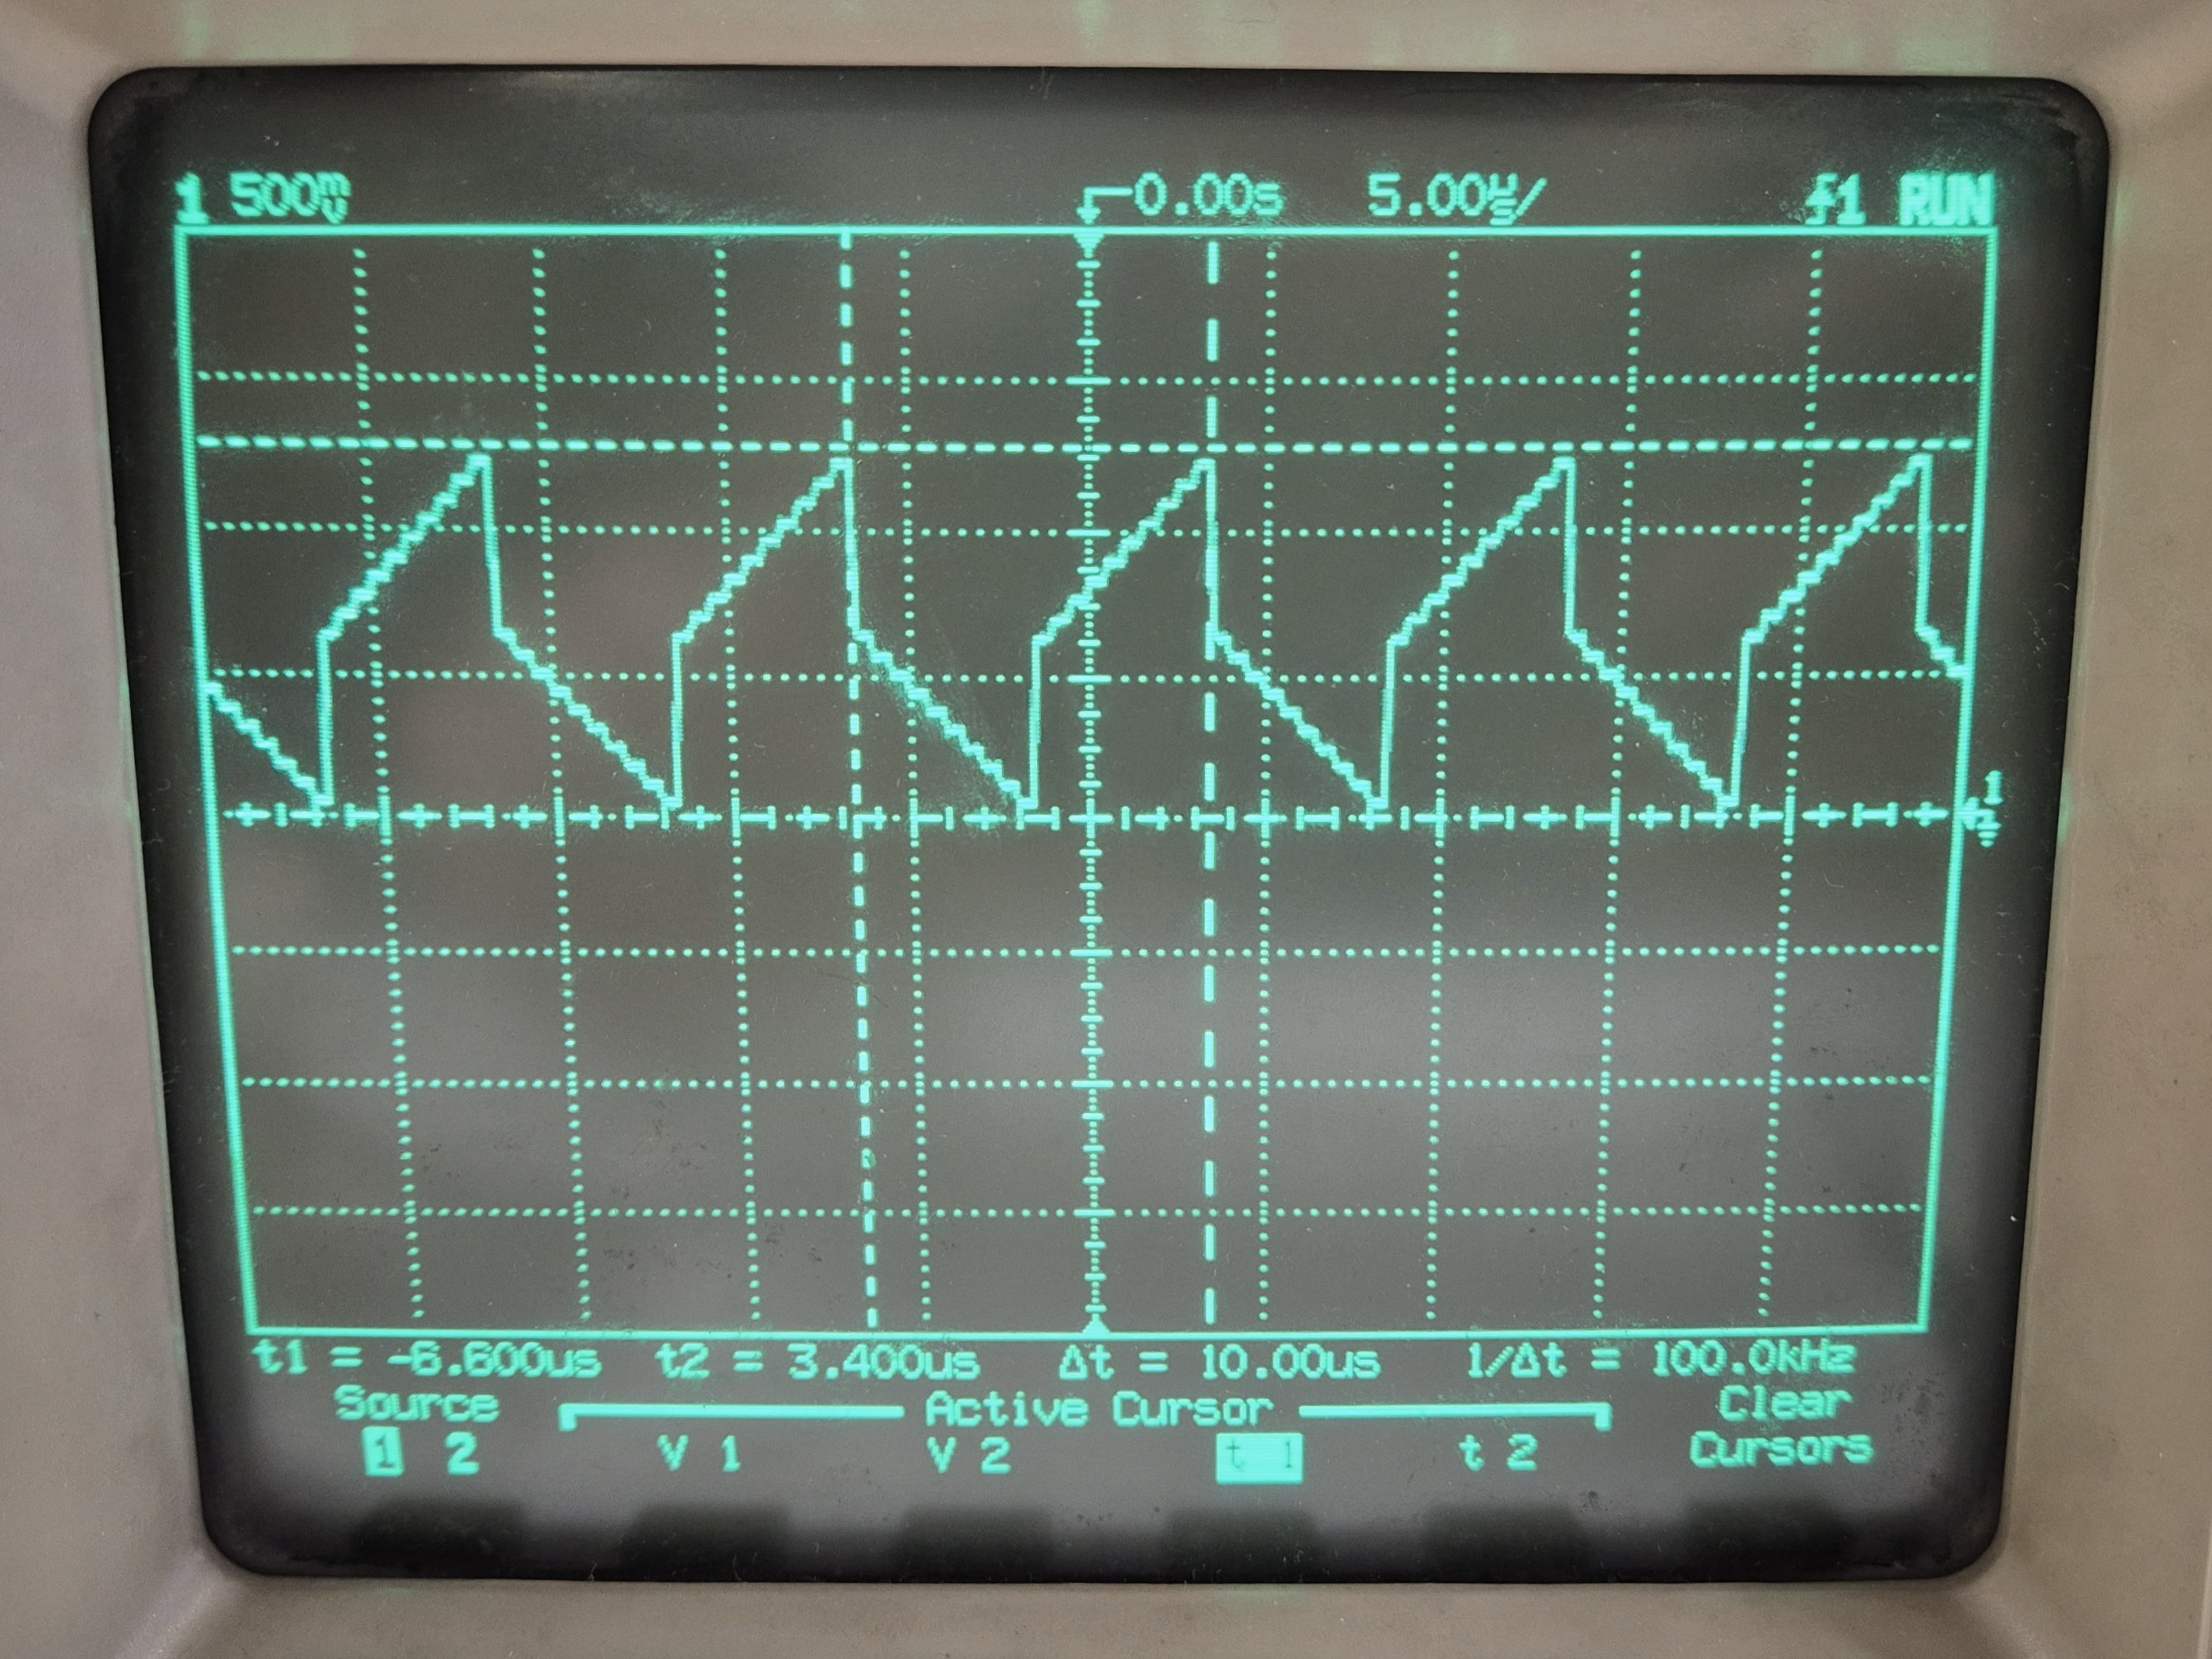
\includegraphics[width=0.8\textwidth]{img/final_test_img6.jpg}
    \caption{Quarter triangular x mirrored, oscilloscope view}
    \label{fig:final_test_img6}
\end{figure}

\newpage
\noindent
Another test that was conducted verified that the signal from the keypad module becomes increasingly difficult to read as the scan rate increases, until it becomes impossible to read at a clock rate of \(50 MHz\).

\vspace{0.5cm}
\begin{figure}[h!]
    \centering
    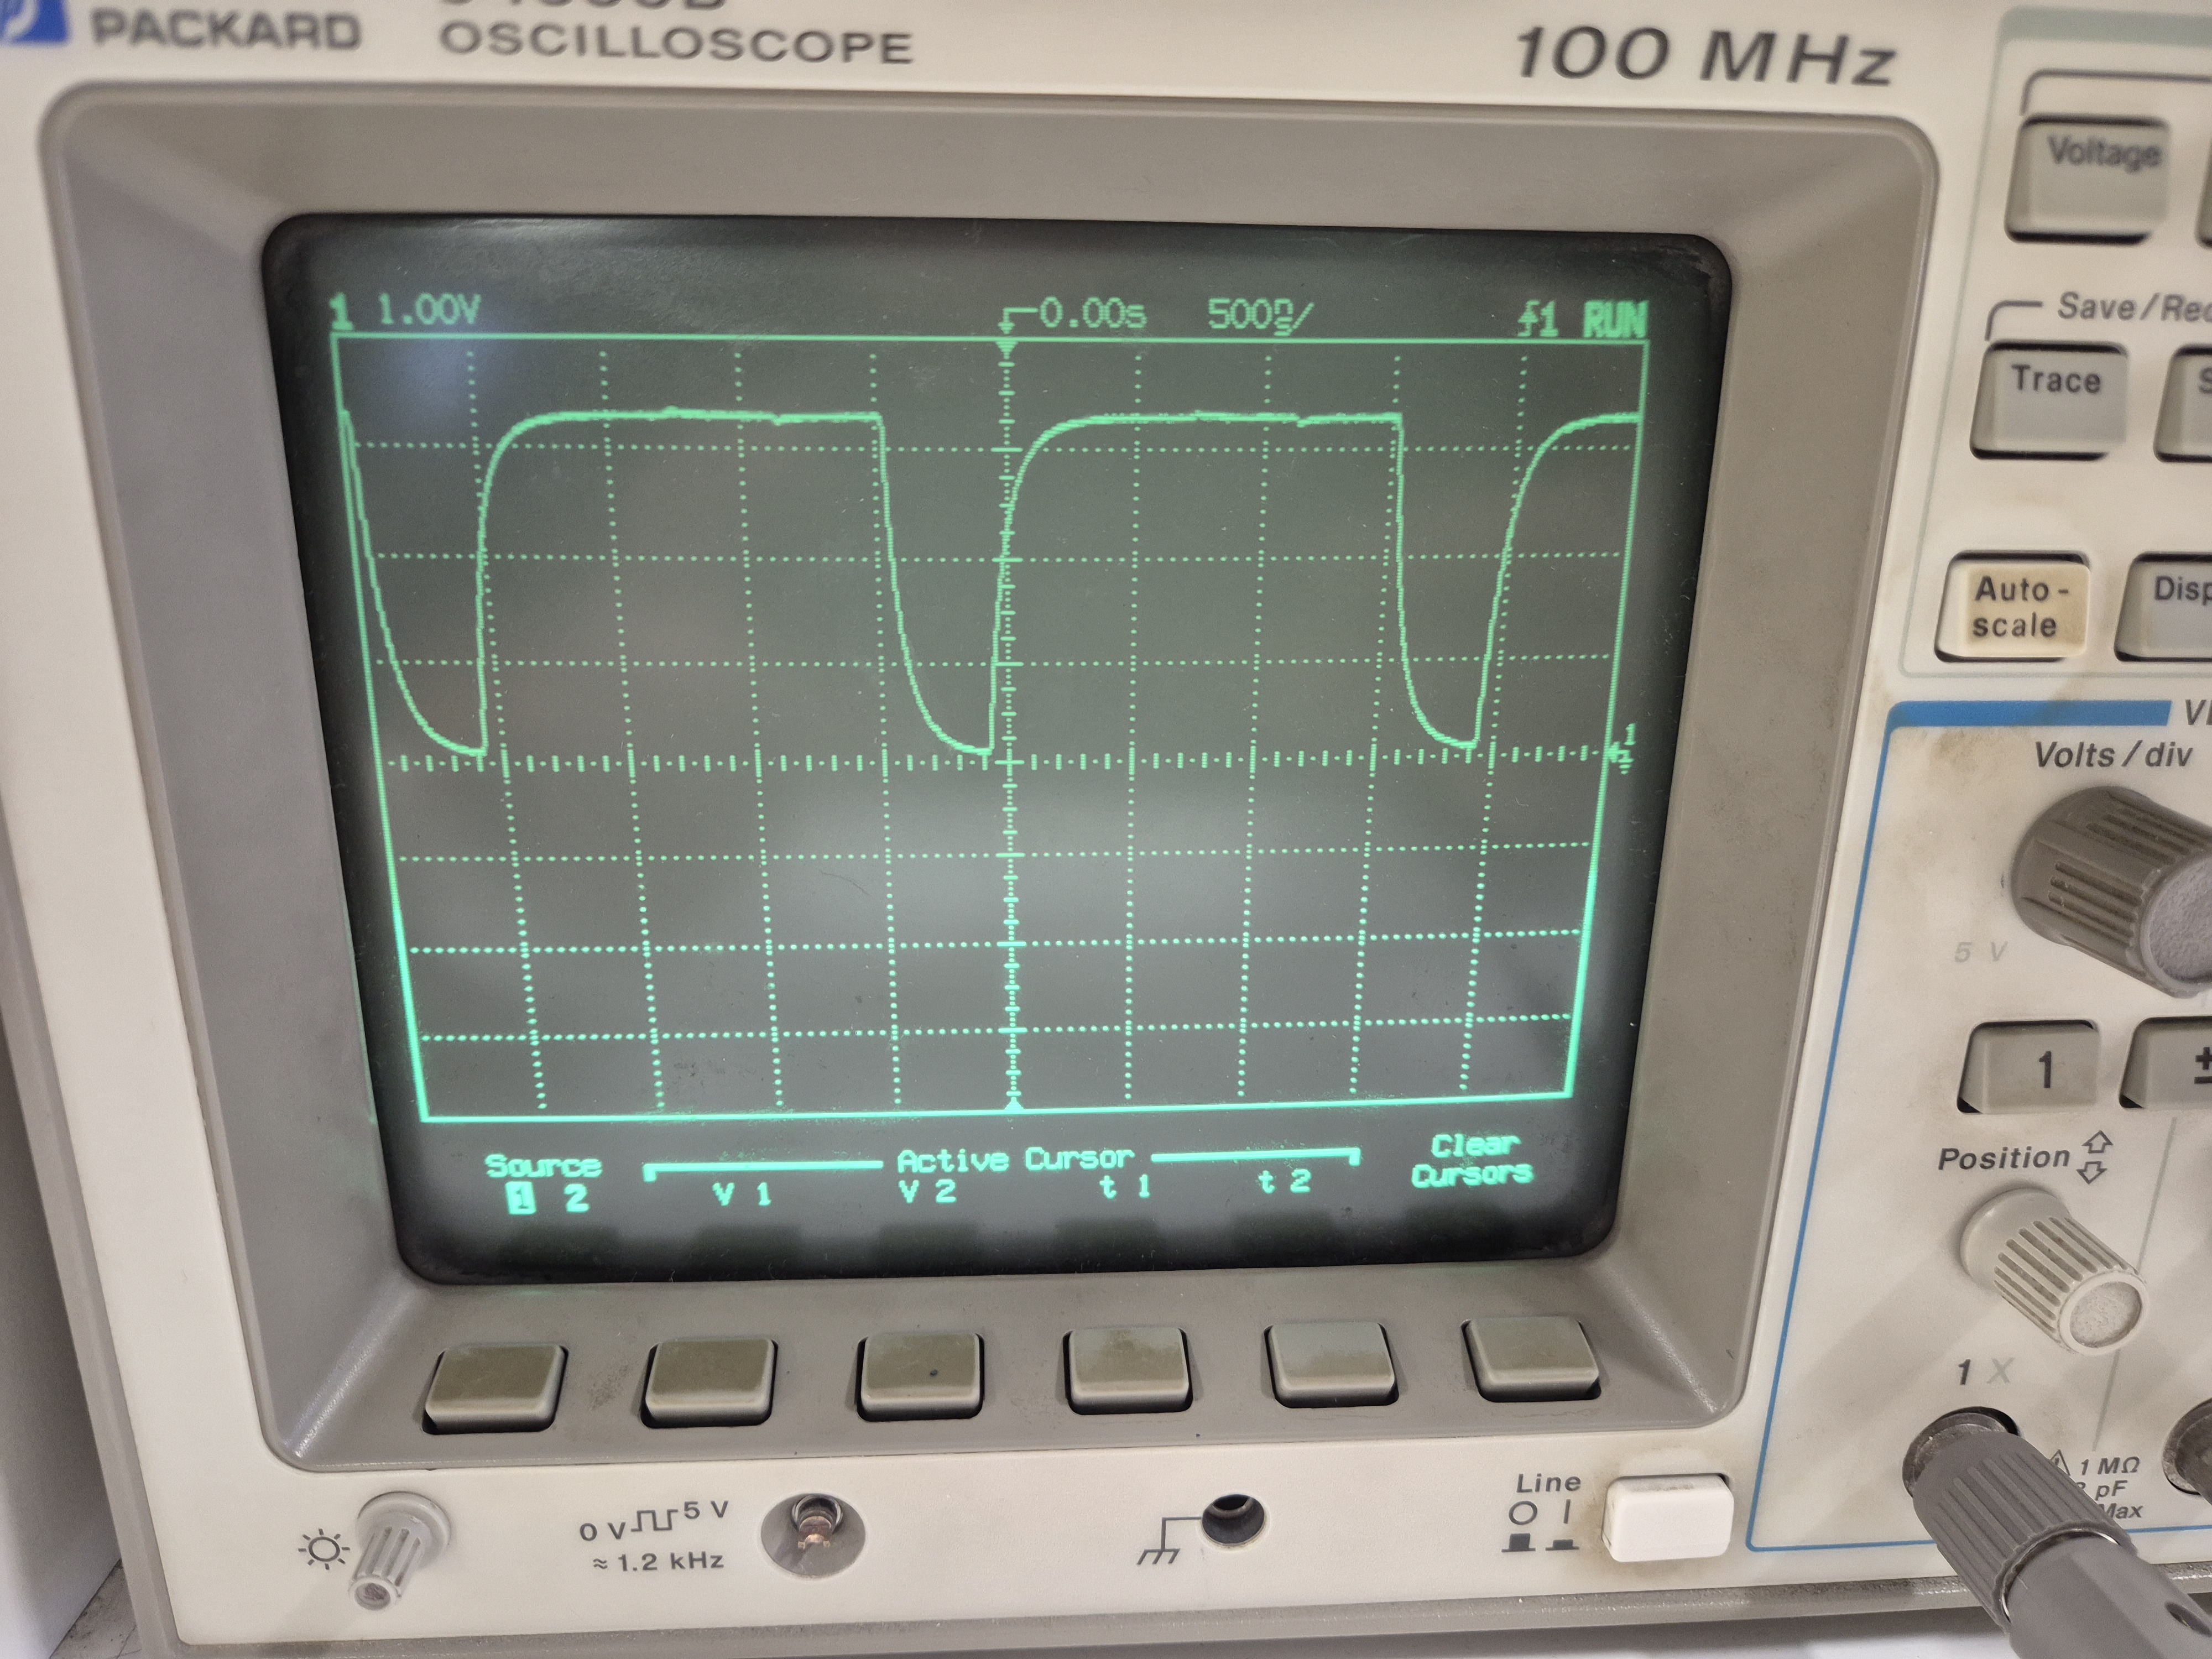
\includegraphics[width=0.8\textwidth]{img/5MHz_keypad.jpg}
    \caption{Signal read from the keypad with a scan frequency of 5MHz}
    \label{fig:5MHz_keypad}
\end{figure}

\begin{figure}[h!]
    \centering
    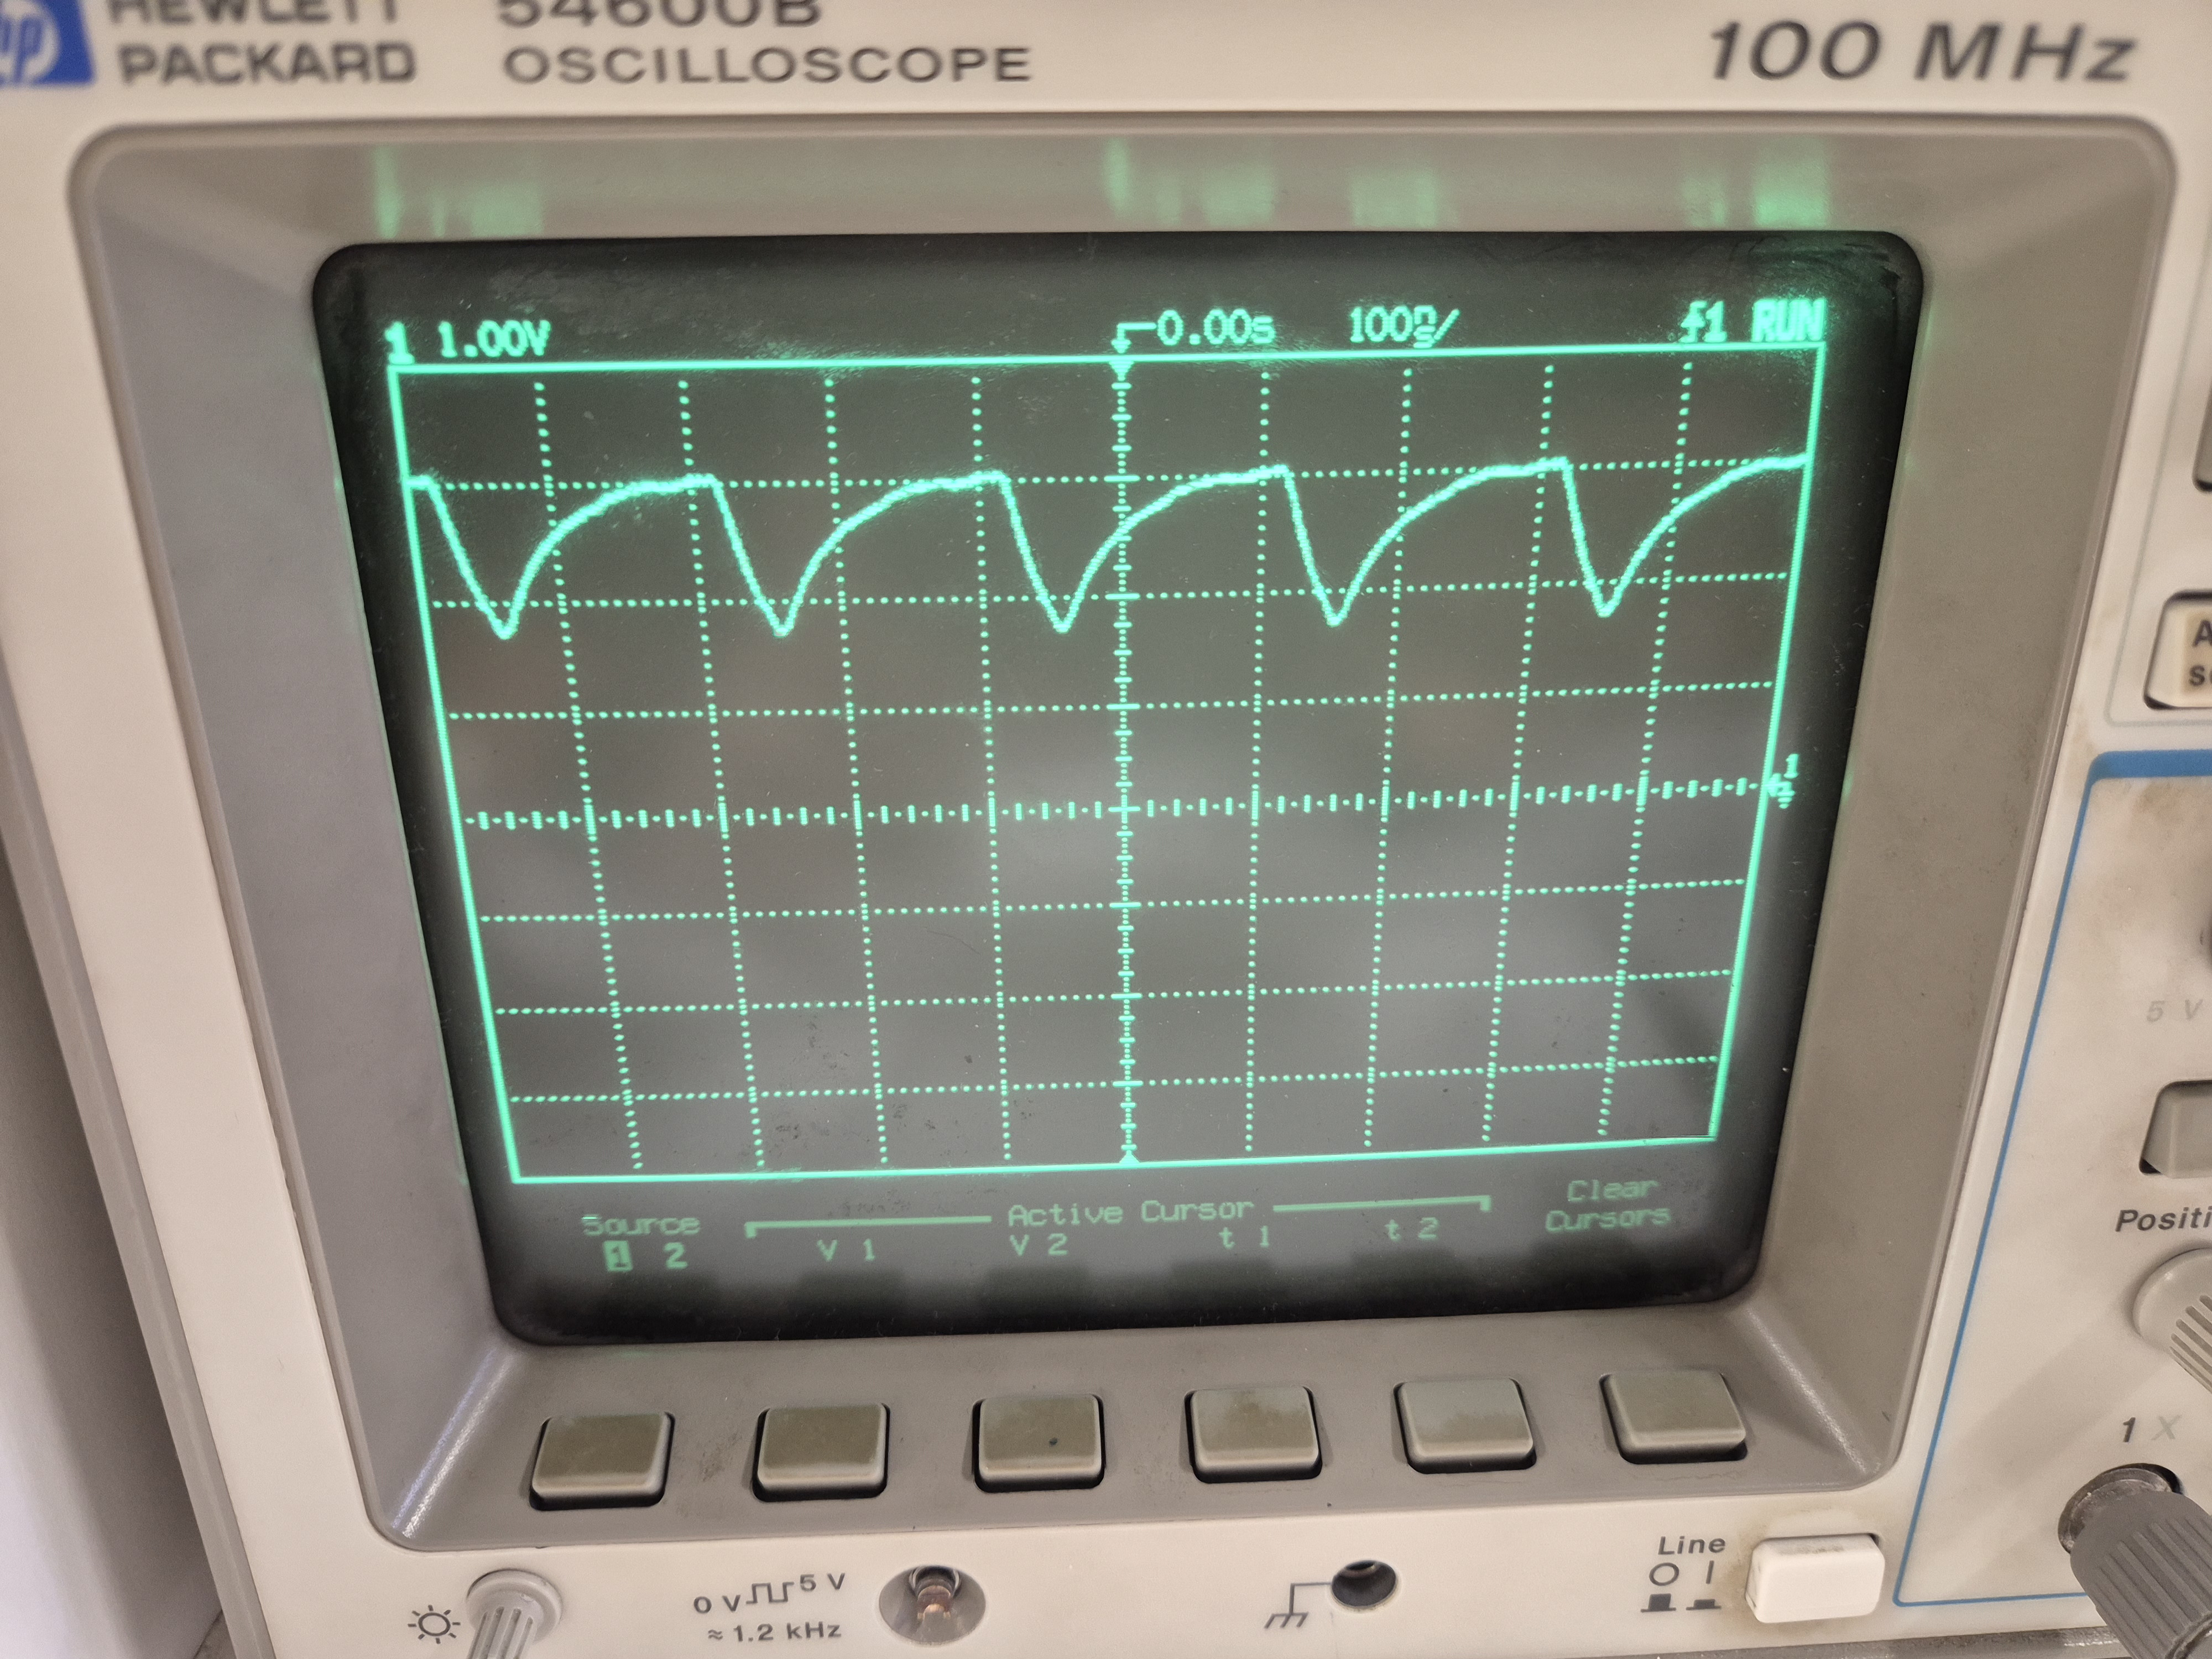
\includegraphics[width=0.8\textwidth]{img/50MHz_keypad.jpg}
    \caption{Signal read from the keypad with a scan frequency of 50MHz}
    \label{fig:50MHz_keypad}
\end{figure}
